%%%%%%%%%%%%%%%%%%%%%%%%%%%%%%%%%%%%%%%%%%%%%%%%%%%%%%%%%%
%
% eXascale Infolab thesis template -- Bachelor and Masters
% version 1.1, Oct 2019
%
%%%%%%%%%%%%%%%%%%%%%%%%%%%%%%%%%%%%%%%%%%%%%%%%%%%%%%%%%%
%
% Based on:
% Masters/Doctoral Thesis
% LaTeX Template Version 2.5 (27/8/17)
% http://www.LaTeXTemplates.com
% CC BY-NC-SA 3.0 (http://creativecommons.org/licenses/by-nc-sa/3.0/)
%
%%%%%%%%%%%%%%%%%%%%%%%%%%%%%%%%%%%%%%%%%

\documentclass[11pt,english,singlespacing,headsepline,consistentlayout]{structure/XI_thesis}

%----------------------------------------------------------------------------------------
%	LATEX PACKAGES
%----------------------------------------------------------------------------------------
\usepackage[utf8]{inputenc} % Required for inputting international characters
\usepackage[T1]{fontenc} % Output font encoding for international characters
\usepackage{mathpazo} % Use the Palatino font by default
\usepackage[backend=bibtex,style=numeric,natbib=true]{biblatex} % Use the bibtex backend with the square citation style (which resembles APA)
\usepackage[autostyle=true]{csquotes} % Required to generate language-dependent quotes in the bibliography
\usepackage{booktabs}       % professional-quality tables
\usepackage{array}          % custom sizes for table columns
\usepackage{amssymb}        % extended blackboard math symbols
\usepackage{amsmath}        % complete AMS math package
% \usepackage[english]{babel} % spelling / syllabification
\usepackage{algorithm}      % pseudocode float
\usepackage[noend]{algpseudocode}  % pseudocode macros
\usepackage{graphicx}       % include graphics
\usepackage{epstopdf}       % vectorial graphics
\usepackage{subcaption}     % sub captions
\usepackage{url}            % URLs

\usepackage{xcolor} % specify custom colours
\usepackage{listings} % code syntax highlighting
\usepackage{newtxmath} % greek symbols

% Load package settings
% !TEX root = ../main.tex

%----------------------------------------------------------------------------------------
% PACKAGE CONFIGURATIONS
%----------------------------------------------------------------------------------------

% Filename of the bibliography
\addbibresource{structure/main.bib}

% Margin settings
\geometry{
  paper=a4paper, % Paper format
  inner=2.5cm, % Inner margin
  outer=3.8cm, % Outer margin
  bindingoffset=.5cm, % Binding offset
  top=1.5cm, % Top margin
  bottom=1.5cm, % Bottom margin
  %showframe, % Uncomment to show how the type block is set on the page
}

% Figures location
\graphicspath{{figures/}}
\DeclareGraphicsExtensions{.pdf,.png,.jpg,.jpeg,.eps,.ps}


% Custom P4 syntax hightlighting
\lstdefinelanguage{P4}{
    morekeywords={ struct, package, header, metadata, parser, transition, state, actions, action, table, key, control, extern, verif, if, else if, else, return, hit, miss, true, false, inout, in, out, exit, and, or, exact, ternary, lpm, range, valid, mask, match_kind },
    emph={void, const, bool, varbit, bit, int, typedef, tuple, enum, apply },
    sensitive=false, % keywords are not case-sensitive
    morecomment=[l]{//}, % l is for line comment
    morecomment=[s]{/*}{*/}, % s is for start and end delimiter
    morestring=[b]" % defines that strings are enclosed in double quotes
}

% P4 syntax hightlighting (use with \begin{P4})
\lstnewenvironment{P4}{
    \colorlet{p4gray}{black!30}
    \colorlet{p4green}{green!60!blue}
    \colorlet{p4key}{brown}
    \colorlet{p4emph}{violet}
    \colorlet{p4mauve}{red!60!blue}
    \lstset{
      backgroundcolor=\color{gray!10},
      basicstyle=\ttfamily,
      columns=fullflexible,
      breakatwhitespace=false,
      breaklines=true,
      captionpos=b,
      commentstyle=\color{p4green},
      extendedchars=true,
      frame=single,
      keepspaces=true,
      keywordstyle=\color{p4key},
      emphstyle=\color{p4emph},
      language=P4,
      numbers=none, % line numbers (left, right or none)
      numbersep=0,
      numberstyle=\tiny\color{blue},
      rulecolor=\color{p4gray},
      showspaces=false,
      showtabs=false,
      stepnumber=1,
      stringstyle=\color{p4mauve},
      tabsize=3,
      title=\lstname
    }
  }
  {}

% C++ syntax hightlighting (use with \begin{C++})
\lstnewenvironment{C++}
  {
    \colorlet{cppgray}{black!30}
    \colorlet{cppgreen}{green!60!blue}
    \colorlet{cppmauve}{red!60!blue}
    \lstset{
      backgroundcolor=\color{gray!10},
      basicstyle=\ttfamily,
      columns=fullflexible,
      breakatwhitespace=false,
      breaklines=true,
      captionpos=b,
      commentstyle=\color{cppgreen},
      extendedchars=true,
      frame=single,
      keepspaces=true,
      keywordstyle=\color{blue},
      language=c++,
      numbers=none,
      numbersep=5pt,
      numberstyle=\tiny\color{blue},
      rulecolor=\color{cppgray},
      showspaces=false,
      showtabs=false,
      stepnumber=5,
      stringstyle=\color{cppmauve},
      tabsize=3,
      title=\lstname
    }
  }
  {}

% !TEX root = ../main.tex

%----------------------------------------------------------------------------------------
% THESIS INFORMATION
%----------------------------------------------------------------------------------------

\thesistitle{Two layer RMIs on P4 capable network switches} % Your thesis title, this is used in the title and abstract, print it elsewhere with \ttitle
\supervisor{Prof. Dr. Philippe Cudré-Mauroux} % Your supervisor's name, this is used in the title page, print it elsewhere with \supname
\cosupervisor{Dr. Alberto Lerner} % If you have a co-supervisor, include it here. This is used in the title page, print it elsewhere with \supname
\degree{Bachelor} % Your degree name, this is used in the title page and abstract, print it elsewhere with \degreename
\author{Lucas Bürgi} % Your name, this is used in the title page and abstract, print it elsewhere with \authorname
\addresses{Bd de Pérolles 90} % Your address, this is not currently used anywhere in the template, print it elsewhere with \addressname

\subject{Computer Science} % Your subject area, this is not currently used anywhere in the template, print it elsewhere with \subjectname
\keywords{SOSD, Learned Index Structures, RMI, P4, Network Programmability, BMv2, Mininet, IEEE754, Floating Point Arithmetic} % Keywords for your thesis, print it with \keywordnames
\university{\href{http://www.unifr.ch}{University of Fribourg}} % Your university's name and URL, this is used in the title page and abstract, print it elsewhere with \univname
\department{\href{https://www3.unifr.ch/inf/fr/}{Department of Informatics}} % Your department's name and URL, this is used in the title page and abstract, print it elsewhere with \deptname
\group{\href{https://www3.unifr.ch/inf/en/exascale-infolab.html}{eXascale Infolab}} % Your research group's name and URL, this is used in the title page, print it elsewhere with \groupname
\faculty{\href{https://www3.unifr.ch/scimed/fr/}{Faculty of Science and Medicine}} % Your faculty's name and URL, this is used in the title page and abstract, print it elsewhere with \facname


\AtBeginDocument{
  \hypersetup{pdftitle=\ttitle} % Set the PDF's title to your title
  \hypersetup{pdfauthor=\authorname} % Set the PDF's author to your name
  \hypersetup{pdfkeywords=\keywordnames} % Set the PDF's keywords to your keywords
}

%----------------------------------------------------------------------------------------
\begin{document}
\frontmatter
\pagestyle{plain}

% !TEX root = ../main.tex

%----------------------------------------------------------------------------------------
% TITLE PAGE
%----------------------------------------------------------------------------------------

\begin{titlepage}
\begin{center}

%\includegraphics[width=15cm]{logos/xi_logos}
%\vspace*{.06\textheight}
%\\

\begin{figure}
  \centering
    
\includegraphics[width=.17\textwidth]{logos/unifr_logo}
  \hfill
    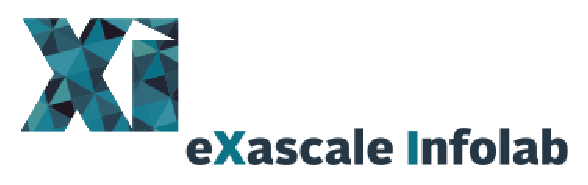
\includegraphics[width=.4\textwidth]{logos/xi_logo}
  \vspace{30mm}
\end{figure}

{\scshape\LARGE \univname\par}\vspace{1.5cm} % University name
\textsc{\Large Bachelor Thesis}\\[0.5cm] % Thesis type
\HRule \\[0.4cm] % Horizontal line
{\huge \bfseries \ttitle\par}\vspace{0.4cm} % Thesis title
\HRule \\[1.5cm] % Horizontal line

\begin{minipage}[t]{0.4\textwidth}
\begin{flushleft} \large
\emph{Author:}\\
\href{mailto://lucas.buergi@unifr.ch}{\authorname} % Author name - remove the \href bracket to remove the link
\end{flushleft}
\end{minipage}
\begin{minipage}[t]{0.4\textwidth}
\begin{flushright} \large
\emph{Supervisor:} \\
\href{https://exascale.info/phil}{\supname} % Supervisor name - remove the \href bracket to remove the link
\\\vspace*{1ex}\emph{Co-Supervisor:} \\ % Remove these two lines if no co-supervisor is involved
\href{https://exascale.info/members/}{\cosupname} % Co-supervisor name - remove the \href bracket to remove the link
\end{flushright}
\end{minipage}\\[1cm]

January 01, 2022 % date of the official defense
\vspace*{.06\textheight}

%\large \textit{A thesis submitted in fulfillment of the requirements\\ for the degree of \degreename}\textit{ in the}\\[0.3cm] % University requirement text
\groupname\\\deptname\\ % Research group name and department name
\vfill

\footnotesize{ Boulevard de Pérolles 90 ~~$\bullet$~~ 1700~Fribourg ~~$\bullet$~~ Switzerland
            \\
            phone +41~(26)~300~84~65 ~~$\bullet$~~ \textsf{diuf-secr@unifr.ch} ~~$\bullet$~~ \textsf{www3.unifr.ch/inf}
            }


\end{center}
\end{titlepage}
 % Title page definition
% Include declaration page -- not necessary for Bachelor and Masters
% % !TEX root = ../main.tex

%----------------------------------------------------------------------------------------
% DECLARATION PAGE
%----------------------------------------------------------------------------------------

\begin{declaration}
\addchaptertocentry{\authorshipname} % Add the declaration to the table of contents
\noindent I, \authorname, declare that this thesis titled, \enquote{\ttitle} and the work presented in it are my own. I confirm that:

\begin{itemize}
\item This work was done wholly or mainly while in candidature for a research degree at this University.
\item Where any part of this thesis has previously been submitted for a degree or any other qualification at this University or any other institution, this has been clearly stated.
\item Where I have consulted the published work of others, this is always clearly attributed.
\item Where I have quoted from the work of others, the source is always given. With the exception of such quotations, this thesis is entirely my own work.
\item I have acknowledged all main sources of help.
\item Where the thesis is based on work done by myself jointly with others, I have made clear exactly what was done by others and what I have contributed myself.\\
\end{itemize}

\noindent Signed:\\
\rule[0.5em]{25em}{0.5pt} % This prints a line for the signature

\noindent Date:\\
\rule[0.5em]{25em}{0.5pt} % This prints a line to write the date
\end{declaration}

\cleardoublepage

%----------------------------------------------------------------------------------------
%	QUOTATION PAGE
%----------------------------------------------------------------------------------------
% Include only in the final submission, after the defense and all required corrections
%\vspace*{0.2\textheight}
%\noindent\enquote{\itshape Quote here}\bigbreak

%----------------------------------------------------------------------------------------
%   ABSTRACT PAGE
%----------------------------------------------------------------------------------------
\begin{abstract}
\addchaptertocentry{\abstractname} % Add the abstract to the table of contents
% !TEX root = ../main.tex
Recently several works proposed new approaches on how advancements in machine learning can be used to improve indexing strategies on sorted data. This led to the SOSD benchmark \cite{sosd-vldb} which enabled having a baseline for evaluating different competitors in a standardized way. At the same time, with a wider adoption of network programmability through P4, a trend towards outsourcing computationally intensive procedures to programmable switches started. Our goal is to combine these two advancements by maintaining recent progress that learned indexing algorithms offer and evaluate possibilities of further leveraging their performance by using the power of network programmability.\\

After careful evaluation we come to the decision that we continue our work focusing on the learned indexing algorithm RMI \cite{rmi}, which suits our idea of implementing parts of it over the network best. Indeed we find that the P4 specification \cite{p4-spec} allows an implementation of the lookup part of RMI on the switch and attains perfect accuracy when tested on virtually simulated network hardware. At this point we analyze how far away our theoretical implementation is, from actually running on real world hardware and we find that there is a long way to go. From this result we then generalize our solution to any dataset and arbitrary RMI configuration by adapting the code generation part of the RMI reference implementation \cite{cdfshop} to output P4 source code files. We finally conclude our work by coming up with a strategy to, even though having a theoretical implementation, estimate how much our idea of outsourcing RMI calculations to the network could benefit a closed system. We find that we could save around 50-100ns per lookup per last mile search worker, which would result in a constant speed up that scales horizontally with the amount of last mile search workers available to a single switch.

\vfill
\begin{center}
\textbf{Keywords:}~\keywordnames
\end{center}
\end{abstract}

%----------------------------------------------------------------------------------------
%	LIST OF CONTENTS/FIGURES/TABLES + TRANSITION PAGES
%----------------------------------------------------------------------------------------
\hypersetup{linkcolor=black}
\tableofcontents % Prints the main table of contents
\listoffigures % Prints the list of figures
\mainmatter % Begin numeric (1,2,3...) page numbering
\pagestyle{thesis} % Return the page headers back to the "thesis" style

%----------------------------------------------------------------------------------------
%	THESIS CONTENT - CHAPTERS
%----------------------------------------------------------------------------------------
% !TEX root = ../main.tex

\chapter{Introduction}
\label{ch:introduction}
This work started by setting up the SOSD benchmark \cite{sosd-neurips} on a local system, with the premise in mind that learned index structures potentially can outperform traditional index structures. Part of this process would be to verify the promised results on said local system. After comparable results to the original paper \cite{sosd-neurips} the idea of taking advantage of the benefits that learned index structures offer and fusing these with the now more and more established network programmability offered by P4 became the essential goal of this work.

\section{Motivation}
A network device is usually very good and very fast at specific simple tasks. In other words it can treat an enourmous amount of packets in a very small amount of time. On the down side of things though it is limited in what operations it can offer and how complex a composition of them can get as well as the amount of memory that is at disposal. This becomes interesting when looking the fact that learned index structures tend to work in a way that they have a rather complex learning phase, where quite some time is spent on examining the data and it's nature before then storing the gathered information in some form. The assumption is that the actual lookup then, due to the previous processing, should now be relatively simple and especially computationally cheap. Further, learned index structures are often capable of adapting the amount of memory they consume depending on the requested prediction accuracy defined in the learning phase. Prediction accuracy in this context means that the predicted bound returned from the learned index structure encloses the actual key more closely or not. This results in a memory to prediction accuracy tradeoff that could potentially be interesting for devices with limited memory capabilities. Another important aspect is that lately hardware acceleration through the efficient usage of secondary devices with some sort of computational power (like switches, NICs, SSD drives, etc.) has become a key aspect for making (distributed) systems faster. In terms of networks this was mainly allowed through a wider adoption of the P4 language.\\

In general the motivation for this work is to potentially speed up all sorts of operations that require lookups on sorted data by allowing them to satisfy their requests directly through the network. With that in mind this work tries to explore the actual feasibility and possibilities that a suitable learned index structure could offer when implemented on a P4 capable network device.\pagebreak

\section{Thesis structure}
In chapter 2, an overview of what techniques and resources were used and tested is given, as well as which ones and why some of them where finally further pursued.\\

\noindent
In chapter 3, a potential implementation of a two-layer RMI on the synthetic BMv2 switch is proposed as well as an evaluation on how far away current physical switches are from what would be needed.\\

\noindent
In chapter 4, an adaptation of the reference RMI implementation \cite{cdfshop} to be able to generate P4 source code files is presented.\\

\noindent
In chapter 5, some additional measurements are made and combined with hypothetical calculations of what switches are theoretically capable of doing today to try to get an approximate idea of how fruitful this work could be in the future.\\

\noindent
Finally in chapter 6 this thesis is closed by stating our conclusions and looking at potential future work.

% !TEX root = ../main.tex

\chapter{Background}
\label{ch:background}
This chapter describes the steps involved in order to determine which learned index structure was worth the effort of further exploration. As a starting point, this was achieved by running and evaluating the SOSD benchmark \cite{sosd-neurips} on a local system. Further, as a second indicator, by looking at what different learned index structures make use of in terms of complexity during their learning phases or more importantly what level of complexity and what programming concepts are needed during a lookup.\\

Finally this chapter looks at the basic capabilities and limitations of the P4 language, especially in regard to what the language offers that could be used as an advantage for learned index structures or on the other hand which important concepts are potentially missing.

\section{SOSD}
In this first section the goal is to analyse the results of the SOSD benchmark. To that end our work consisted of comparing our local results with what is given by the authors in Table 2 in their paper \cite{sosd-neurips}, which gave the result shown in Figure \ref{fig:sosd_lookups}. It is important to mention for these figures that in order to obtain these results, the benchmark runs different pareto runs for each algorithm on each dataset from which we select the optimal run with respect to the three metrics: lookup time, build time and index size. At this point in time it was important for this work to take note of the fact that when tuned properly, learned index structures effectively \emph{can} outperform traditional index structures with respect to the lookup time metric. When considering the remaining metrics, this results in a tradeoff between either slower lookup times but no build time, or instead spending time on building, as pointed out in Figure \ref{fig:sosd_builds}, to then gain with faster lookups.

\begin{figure}[!ht]
\centering
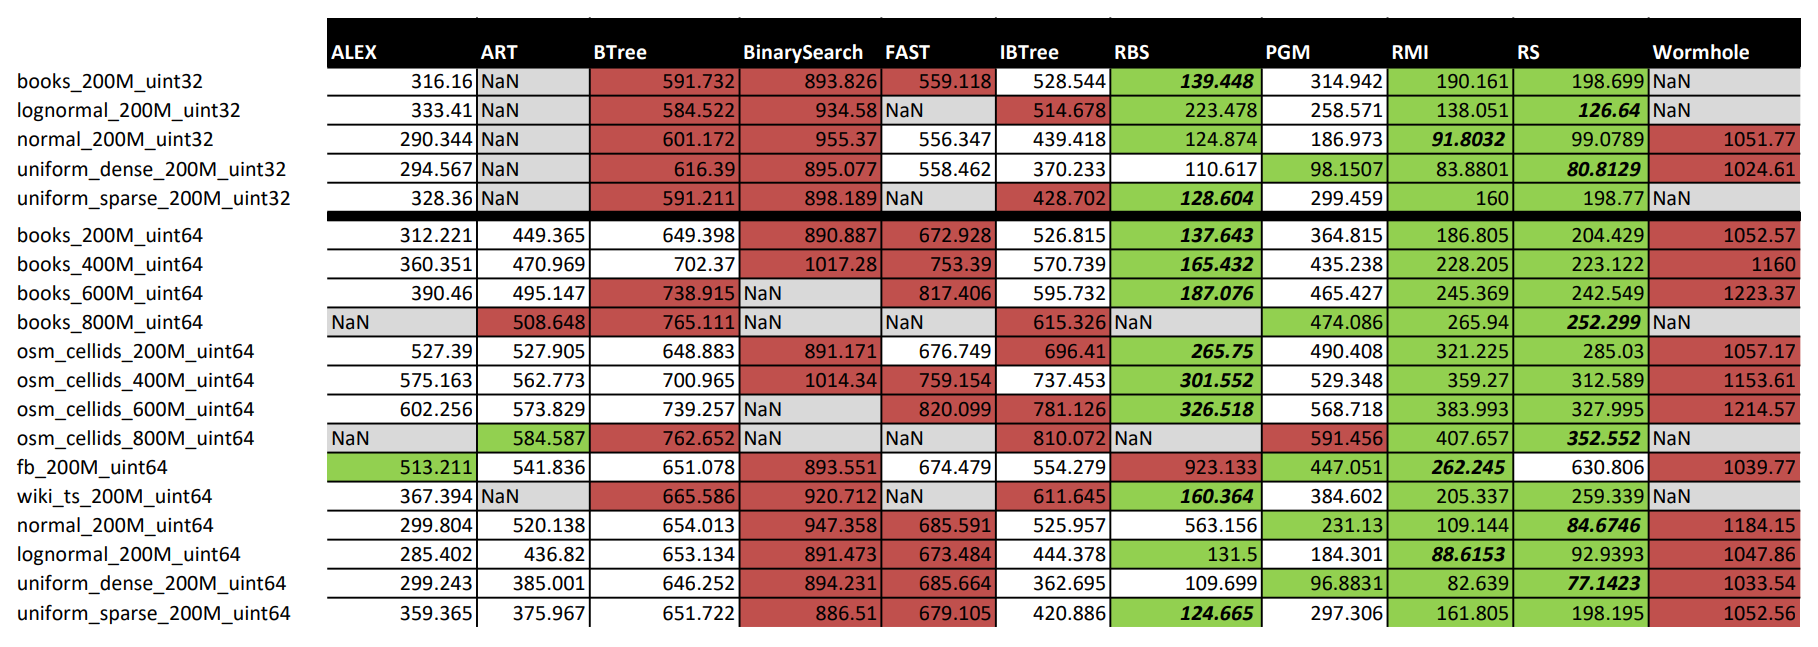
\includegraphics[width=1\textwidth]{sosd_lookups}
\caption[SOSD Lookups]{
  \textbf{SOSD lookup times (in ns).}
  Lookup times produced by the benchmark when installed on our local test machine, selecting the best performing run with respect to the three metrics lookup time, build time and index size among all pareto runs.
}
\label{fig:sosd_lookups}
\end{figure}

\begin{figure}[!ht]
\centering
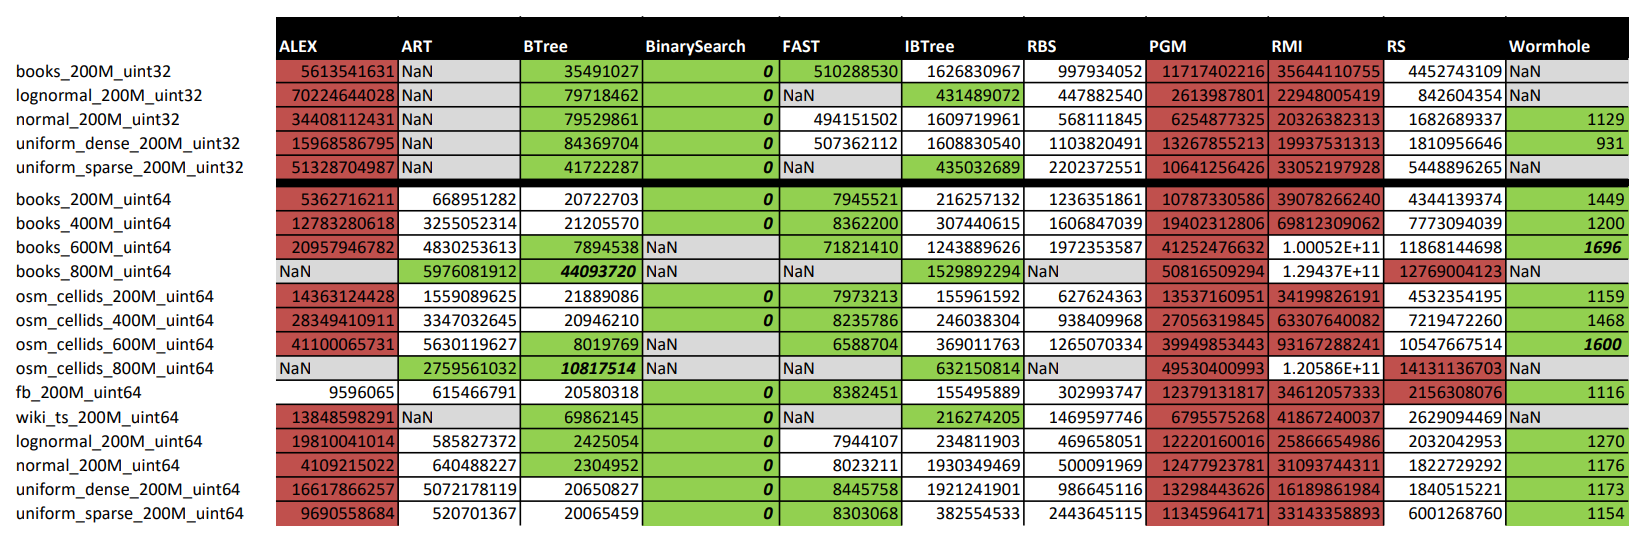
\includegraphics[width=1\textwidth]{sosd_builds}
\caption[SOSD Build Times]{
  \textbf{SOSD build times (in ns).}
  Build times produced by the benchmark selected among pareto runs the same way as above.
}
\label{fig:sosd_builds}
\end{figure}

\begin{figure}[!ht]
\centering
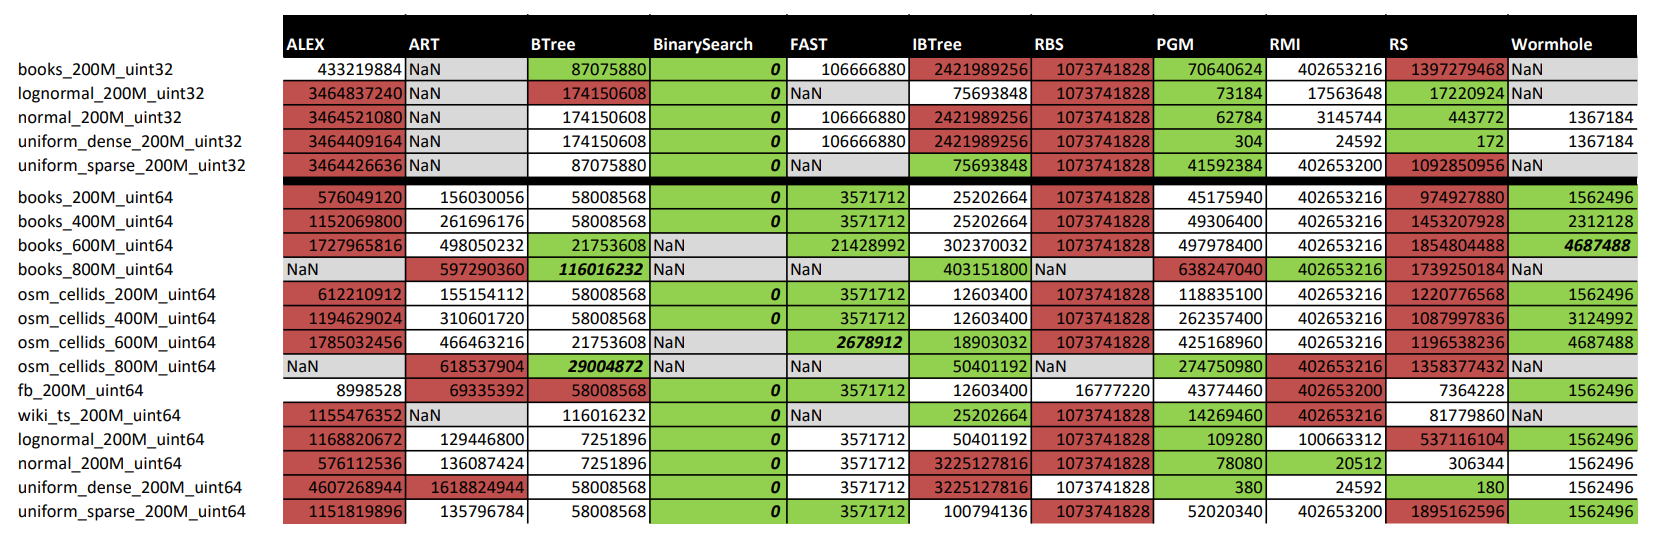
\includegraphics[width=1\textwidth]{sosd_sizes}
\caption[SOSD Index Sizes]{
  \textbf{SOSD index sizes (in bytes).}
  Index sizes produced by the benchmark selected among pareto runs the same way as above.
}
\label{fig:sosd_sizes}
\end{figure}

\section{Learned index structures}
In the SOSD benchmark there are currently three main competitors that belong to the category of learned index structures. Namely, these are RMI, RS and PGM. RMI (Recursive Model Indexes) is proposed in \cite{rmi} and implemented for the benchmark in \cite{cdfshop}. RS (Radix Spline) is proposed and implemented by the original authors in \cite{radixspline}. Finally the same holds for PGM (Piecewise Geometric Model), which is proposed and implemented in \cite{pgm}.

\subsection{RMI: Recursive Model Indexes}
\label{sect:background:rmi}
RMI \cite{rmi} is a learned index structure that is based on the idea that different models fit certain data better. By having a number of different models to choose from during the learning phase and by allowing to stack different models on top of each other in different layers, RMI should adapt well to mostly any given shape of sorted data. In the context of the benchmark as well as in the context of this work, RMIs are fixed to two layers since this proved to be most efficient for most datasets and also reduces complexity for further chapters. In the reference implementation \cite{cdfshop} C++ source code files are generated that contain parameters as well as the adapted code depending on which models were chosen on which layer. Generally the input key is given as input to a first layer, which generates an index that then serves as a starting point for the next layer, and so on, until finally a last layer retrieves the key's estimated position together with a stored error margin.\\

Notable for a potential P4 implementation here is that RMI is using floating point arithmetic, solely focussed on using the floating point FMA instruction. This immediately makes it a big challenge to think about implementing RMI in P4 but leaves some hope in the sense that if an FMA operation together with some simple form of floating point arithmetic could be implemented in P4, then RMI quite quickly would become realistic on a P4 device.

\subsection{RadixSpline: A Single-Pass Learned Index}
RS \cite{radixspline} is built on top of the idea of fitting a linear spline to the CDF function of some sorted data. Different spline segments are indexed and to each segment two spline points are stored. Upon lookup, the learned index tries to locate the responsible spline segment and performs a linear interpolation between the two spline points to find the estimated key position.\\

For P4 programmability important is that RS stores the spline points in floating point format, and upon lookup performs mathematical operations on these floating point numbers. The most notable operations in this context are the calculation of the slope of a spline segment which involves a floating point division and finally the interpolation itself which involves a floating point FMA instruction. This again makes it quite a big challenge to even start thinking about an RS implementation in P4. In comparision to RMI, a big downside of RS is the part where the lookup code tries to locate the responsible spline segment. To make sure the correct segment is chosen either a linear search on small ranges or a binary search on bigger ranges is used. Both search concepts involve conditional iteration over dynamic data and are, to the best of my current knowledge, not feasible in P4.

\subsection{PGM: The Piecewise Geometric Model index}
PGM \cite{pgm} is a pure learned index structure that tries to create a piecewise linear approximation (PLA) that maps keys to their approximate positions in the data with at most $\epsilon$ distance to their actual position. By applying this approximation recursively onto itself multiple levels of PLAs are built such that efficient search becomes possible.\\

The given lookup code in \cite{pgm}, due to its recursive nature at creation, needs to iterate over all levels of PLA for each lookup, which already marks a first challenge. To make things even harder in terms of P4 programmability, on each level of PLA either linear search for small ranges or binary search for bigger ranges is used to determine which PLA is responsible for a given key on the next level. This then results in a very similar situation as for RS, where core concepts used for looking up keys are far from easily feasible in P4 as described in the previous section.

\section{P4 and network programmability}
P4 is a programming language that allows standardized programmability of network devices, especially targeting their packet forwarding planes. The language first appeared in 2013 and is since maintained by the P4 language consortium. Personally, I was introduced to this language through my supervisor and further learned some of the basic concepts through the publicly available records of the P4 Developer Day \cite{p4-devday}. Another important source for a deeper understanding of what the P4 language offers and which limitations exist is via the official specification \cite{p4-spec}.\\
The idea behind learning P4 is to implement the best fitting of the previously presented learned index structures on a network device to satisfy our goal of resolving lookup requests directly through the network. The following preliminary facts need to be taken into consideration.

\begin{itemize}
  \item The P4 packet flow consists of different pipelines, inlcuding a packet parser, a checksum verification, an ingress pipeline, an egress pipeline, a checksum computation and finally a packet deparser.
  \item Parsers can have different states and allow transitions from state to state. States can loop back to other states but their logic must be reducible to a final state machine at compilation time, meaning there is no dynamic form of recursion or iteration allowed (The only exception to this are header stacks where a packet can contain a dynamic but only up to a fixed amount of stack items that can be extracted through state recursion).
  \item There are match-action tables that can optionally be filled with data from the control plane during runtime via P4Runtime \cite{p4runtime-spec}. Tables allow matches on keys and execution of some specific action depending on the match.
  \item There is no possibility of linking P4 source code files to each other similar as for example in C. This creates an environement where no major libraries exist, at most code snippets could be used.
  \item There is no notion of floating point numbers or floating point arithmetic. The concepts do simply not exist in P4 land.
\end{itemize}

All together, this leads to a very interesting language by itself but also to a rather cumbersome discovery of everything that is actually not possible. Namely this includes, especially with regard to what different learned index structure implementations require, that in P4 there is no floating point arithmetic and there is no sort of dynamic loop or recursion capability.

% !TEX root = ../main.tex

\chapter{RMI on BMv2}
\label{ch:rmionbmv2}

The next chapter of this work is dedicated to the idea of implementing RMI using the reference P4 software switch BMv2. As briefly described in section \ref{sect:background:rmi}, a RMI lookup heavily relies on floating point arithmetic but besides that does not need a lot of other operations to work properly. Therefore a major part of this chapter will be about dealing with these floating point operations. For a simpler start as well as for learning a lot of the basics of the P4 language the BMv2 software switch is used. This does bring quite a lot of advantages to begin with, but as decribed later in section \ref{sect:rmionbmv2:evaluation} does also lead to a large differences between what is doable in theory in software and what is actually possible in a real world scenario.

\section{BMv2 and Mininet}
BMv2 stands for behavioral model version two and is the official reference P4 software switch implementation found at \cite{bmv2}. It is written in C++ and can take in and interpret a compiled P4 program and simulate the packet-processing behaviour specified in said P4 program. The implementation runs out of the box on traditional linux distributions and can be combined with virtual network simulation softwares such as \cite{mininet}. Altogether though with regard to this work, neither BMv2 nor Mininet are meant to be production-grade implementations in their area. This means that there are on one side in the case of BMv2 a lot less restrictions imposed than a real world switch would and on the other side for both tools there is a lot less processing speed and throughput potential available than real world equipment would provide.\\

With that out of the way the network architecture simulated by Mininet is extremely simple and barely even worth mentioning. Figure \ref{fig:network_architecture}, in the next section, shows our simple setup and where the BMv2 software switch comes into play together with more detail about the packet flow.

\section{Network setup and packet structure}
\label{sect:rmionbmv2:network}
When looking at how the SOSD benchmark implementation handles many different algorithms at the same time it becomes apparent that separating a phase where an algorithm can do its processing to return a result bound and on the other hand performing the so called last mile search on this remaining bound is key for most learned competitors. This separation comes in handy since performing an efficient search on a given range of data on a P4 switch is not easily doable as of today and therefore this task remains on the host by choice. This leads to the setup shown in figure \ref{fig:network_architecture}. In principle a host sends a regular ethernet packet containing all the usual fields such as destination and source MAC address to the switch. Importantly though the packet sets the ether type field to a custom value of $0x8008$ and appends a payload containing the desired lookup key and space for the response in form of a field for the guessed position and a field for the expected error calculated during the learning phase as visualized in figure  \ref{fig:packet_structure}. As a next step the switch performs the actual RMI calculations, completes the guessed position and expected error field in the packet and forwards the packet back to the source MAC address. The last step that was previously abstracted away is now performed upon receiving the forwarded response packet on the host, meaning that some sort of last mile search is performed in the interval between \([estimated - error, estimated + error]\) to finally find at which position the initially desired lookup key is to be found.\\

In terms of flexibility there is absolutely no restriction of where to forward the finalized RMI packet containing the estimated position and caluclated error to. There are all sorts of possibilites here to use the full power of P4 and network programmability to achieve combinations of packet forwarding and lookup operations. Annother flexibility is the sort of search that is used on the host on the narrowed down search bound. For this work as well as in the SOSD benchmark a regular form of binary search is used, but for different concrete use cases other algorithms may be preferable.

\begin{figure}[ht]
  \centering
  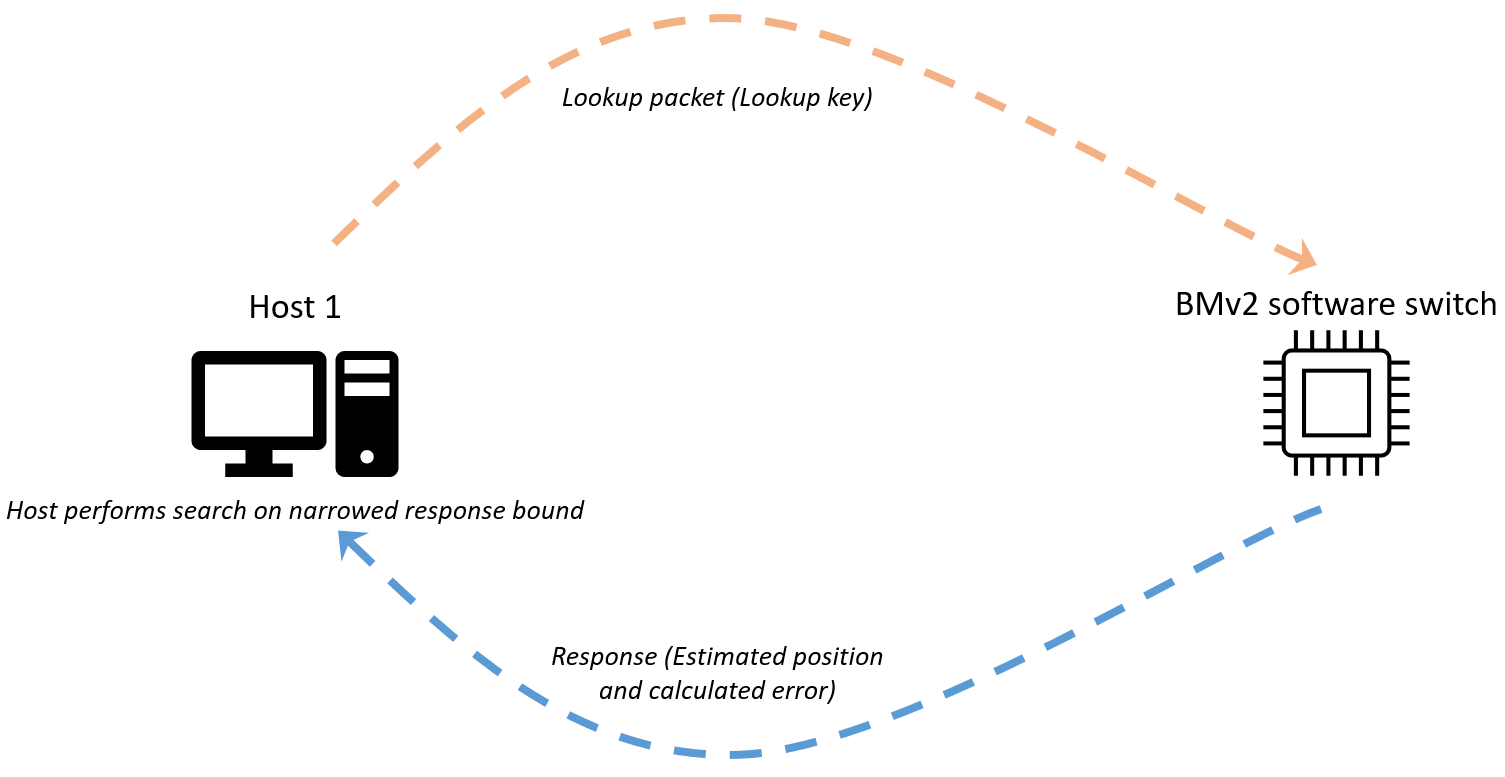
\includegraphics[width=1\textwidth]{network_architecture}
  \caption[Network architecture]{
    \textbf{Mininet network architecture.} Simple network architecture and packet flow proposition to run RMI on a P4 capable switch.
  }
  \label{fig:network_architecture}
\end{figure}

\begin{figure}[ht]
  \centering
  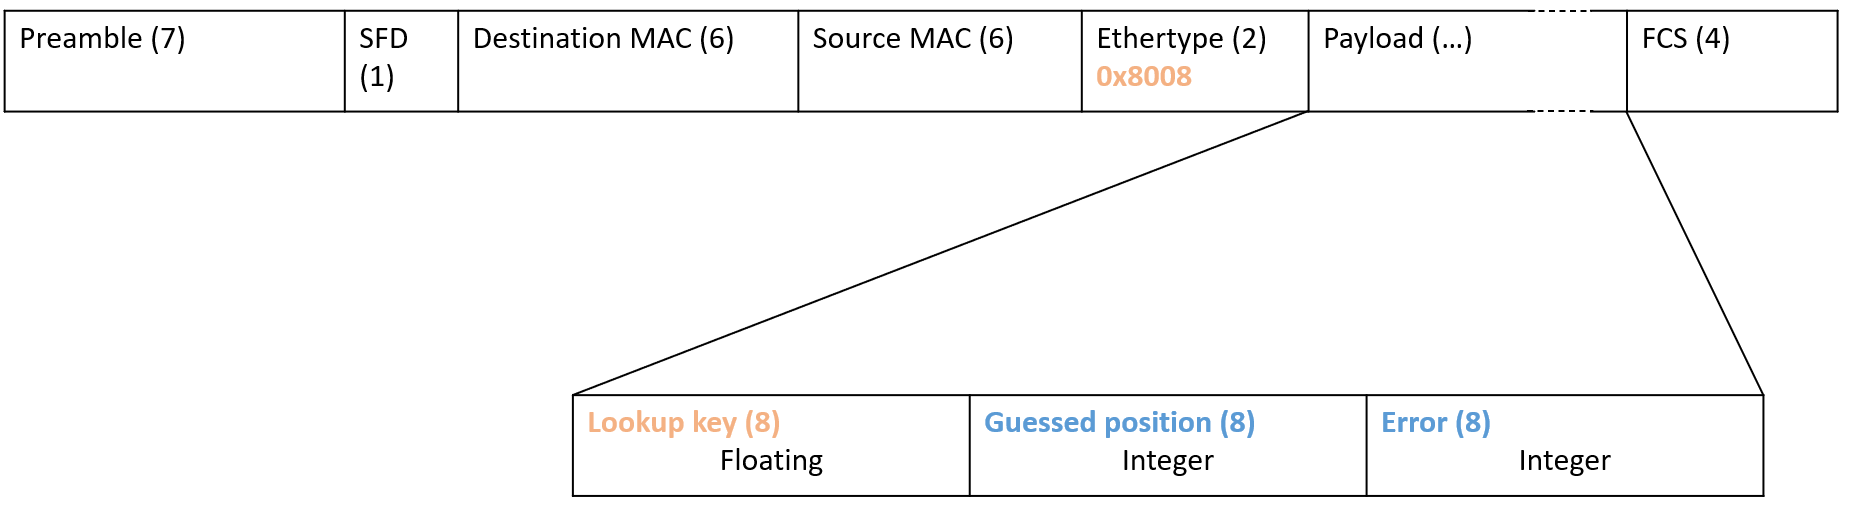
\includegraphics[width=1\textwidth]{packet_structure}
  \caption[RMI packet structure]{
    \textbf{Learned RMI packet structure.} Visualization of an RMI ethernet packet containing the custom ethertype and payload. Field sizes are shown in octets.
  }
  \label{fig:packet_structure}
\end{figure}

\section{Implementation}
\label{sect:rmionbmv2:implmentation}
The reference RMI implementation does generate C++ code depending on the specific dataset it is trained on. This part of the algorithm though is not yet part of this chapter and will be explored more in depth in chapter \ref{ch:rmiforp4}. As a first step to try to translate existing RMI code in C++ into P4 our approach was to decide for a single dataset as well as some constant input parameters. The result of this is that whenever running the existing RMI implementation the exact same C++ code is generated. An example can be found in the appendix in section \ref{sect:appendix:books_200M_uint32_0}. The next step would be to examine the generated code and finally implement the exact same behaviour in P4 by hand. For this multiple challenges must be tackled. One of them being the load function where quite a large chunk of binary layer one parameter data is loaded into memory. Annother one becoming apparent when observing that in this case the learning phase decided for layer zero to use a cubic function and for layer one to use a linear function. The implementations of both of these functions are short as shown in figure \ref{fig:linear_cubic}, but since they solely rely on using the FMA instruction it will turn out that they are going to be quite tricky to translate to P4. In other words a second challenge will be to implement an operation that behaves similarly to the commonly in hardware implemented fused multiply-add CPU instruction in P4.

\captionsetup[figure]{skip=-10pt} % move caption up towards listing
\begin{figure}[ht]
  \begin{C++}
inline double linear(double alpha, double beta, double inp) {
  return std::fma(beta, inp, alpha);
}

inline double cubic(double a, double b, double c, double d, double x) {
  auto v1 = std::fma(a, x, b);
  auto v2 = std::fma(v1, x, c);
  auto v3 = std::fma(v2, x, d);
  return v3;
}\end{C++}
  \caption[Linear and cubic lookup implementation in C++]{ C++ lookup implementation for the linear and cubic model. }
  \label{fig:linear_cubic}
\end{figure}

\subsection{FMA in P4}
\label{sect:rmionbmv2:fma}
This section focusses on a software implementation of the fused multiply-add instruction in P4. The goal is to potentially provide a proof of concept and put performance or optimization considerations aside for now. In section \ref{sect:rmionbmv2:evaluation} a more top down look on things will be given together with some thoughts in form of an evaluation in what way this was a good idea or not.\\

The FMA instruction takes in three parameters and calculates the value resulting from \((x * y) + z\) rounded only once. This means that in order to implement an FMA instruction in P4 one needs to be able to multiply two floating point values as well as adding two floating point values together. This consequently means that there has to be some sort of representation in P4 for a floating point value. This is pretty easily doable by defining a custom header type that follows the official IEEE754 floating point standard published by the \cite{ieee754} shown in figure \ref{fig:double_header}. For 64-bit double values the standard describes a 1-bit field representing the sign, an 11-bit field representing the exponent stored as non-negative biased binary number and finally a 52-bit field representing the mantissa stored as a regular binary number excluding the so called "hidden bit". With this definition set floating point addition as well as floating point multiplication can be addressed.\\

Floating point addition works by first setting the hidden bit on both mantissa fields. Next at its core, by looking at the exponent difference between the two floating point values and shifting the mantissa of the smaller value to the right by that amount. With both mantissas now in the same exponent base, they can be added together with a regular bit addition operation. Lastly both the resulting sign as well as the exponent are determined by the larger floating point value. With this the mathematical addition result is calulcated but the representation is not yet sound, meaning that that due to the calculation the first significant mantissa bit might not be at position 53 where the so called hidden bit is supposed to be. To correct this a normalzation procedure is run where the mantissa and exponent are shifted and adapted such that the first significant mantissa bit moves to position 53 and will finally be omitted to increase the representable value range. In P4 this operation is implemented by ternary matching the calulcated mantissa against a static normalzation table which is shown in a narrowed down form in the appendix in section \ref{sect:appendix:floating_normalization}. The implementation of the addition operation can be found in the appendix in section \ref{sect:appendix:floating_addition}.\\

On the other hand floating point multiplication works similarly by first setting the hidden bit on both mantissa fields. Next, to determine the resulting sign, both input sign bits are XOR-ed together. Further, to determine the resulting exponent, the two unbiased input exponents are added together with a regular bit addition operation. Finally the two mantissa fields are mutliplied together this time with a regular bit multiplication operation and shifted back into their initial exponent space. At this point the mathematical multiplication result is caluclated but again the representation is not yet sound. To correct this the exact same normalzation procedure described in the previous paragraph is run. The implementation of the multiplication operation can be found in the appendix in section \ref{sect:appendix:floating_multiplication}.\\

To finish this section now with both mathematical base operations in place, the final FMA control in P4 does simply execute both of the just described operations one after the other.

\captionsetup[figure]{skip=-10pt} % move caption up towards listing
\begin{figure}[ht]
  \begin{P4}
typedef bit<1> sign_t;
typedef bit<11> exponent_t;
typedef bit<52> mantissa_t;

struct double_t {
  sign_t sign;
  exponent_t exponent;
  mantissa_t mantissa;
}\end{P4}
  \caption[Double header definition in P4]{
    \textbf{IEEE754.} P4 header definition following the IEEE754-2019 standard for 64-bit double values.
  }
  \label{fig:double_header}
\end{figure}

\subsection{Loading model parameters in P4}
With the calculation heavier operations out of the way a next challenge is to have access to the data from the binary file normally directly loaded into memory in C++ representing the so called model parameters that are accessed depending on the resulting calculations of the previous layer. To solve this problem a combination of control plane and data plane is needed. On one side the data plane does predefine an empty table description that later can be filled, while the switch is runnning, from the control plane via the P4Runtime API specified and maintained by \cite{p4runtime-spec}. An example of such a table definition is given in the appendix in section \ref{sect:appendix:rmi_table}. The data plane on the other side now simply reads the existing model parameters file and sends these informations over to the switch. This is done with Python since the P4Runtime environement is implemented in Python. To work correctly the script takes in the location of the binary model parameters file as well as the necessary connection parameters to establish a connection to the switch. The table entries are sent in batches to the switch for acceptable performance in the simlauted network and hardware environement but besides that the implementation is trivial. On the data plane side of things again, whenever a lookup packet arrives and a future layer needs access to model parameters the P4 program performs an exact table match with the reulting index from the previous layer to determine the parameters for the next layer.

\subsection{The actual lookup function}
Finally with the described functions implemented the actual lookup control simply becomes a matter of putting it all together as shown in the appendix in section \ref{sect:appendix:rmi_lookup}. One additional but relatively simple function that had to be implemented was a function that casts a floating point value to an integer in P4. As a basic concept each layer takes in its layer parameters as arguments and returns a prediction index for the next layer. In the example case of the books\_200M dataset with 32-bit keys a two-layer RMI is generated where the first layer follows a cubic model and takes in the statically in the C++ header file (shown in \ref{sect:appendix:books_200M_uint32_0}) present L0 parameters. After doing the FMA calculations for said cubic layer, the result is cast back to an integer which is then used as an index to perform an exact table match with the table described in the previous section to retrieve the L1 parameters used as input for the linear model. Finally the FMA calulations for the linear model are computed and after casting the floating point result back to an integer value, the guessed index is clamped to a value between zero and the dataset size and finally returned.

\section{Evaluation}
\label{sect:rmionbmv2:evaluation}
When running and testing the described setup including the virtual network and the software emulated network switch, the possibilites are obviously very limited. Still though, when looking at accuracy when sending one million test lookups generated by the SOSD benchmark, the P4 implementation on the switch achieves a 100\% prediction accuracy. Meaning for all lookup packets sent, the precomputed lookup key is actually to be found in the range given by the guess and the error returned in the response packet.\\

In any case accuracy is fine and for the scope of this work rather pleasing but the implementation as is does ignore quite a lot of real world limitations. A first one of them being for example that currently available switches do mostly not support multiplication on their ALUs. This does break the floating point multiplication function, which is needed for the FMA implementation which in turn is needed for different model lookup implemenations. Annother one of these limitations being that current real world switches are limited to a certain amount of ALU stages. Meaning that for the switch to reach optimal operation speed, a packet can maximally perform a certain amount of computation. For now since not having any ALU hardware support for floating point arithmetic all mathematical operations are implemented in software and therefore in the current implementation this limit of ALU stages is more than exceeded. A next limitation is discussed in the following section where current switches are very limited in terms of what bit width ALUs can handle for basic operations. A final limitation or moreso a very large negative point comes from the fact that the FMA operation is fully implemented in software. This not only leads to the previously described overfull stage usage but also to bad performace in comparision to hardware implemented FMA instructions on a server's CPU where not only the hardware itself means a significant speed up but also the fact that FMA circuits can often benefit from smarter design choices instead of just performing one mathematical operation after the other.\\

All in all with so much of these limitations on the table, the goal and purpose of this work and of this implemenation definetely and at best becomes a theoretical proof of concept, showing what could potentially be possible. While reaching expected prediction accuracy a lot of progress in terms of extending ALU capability on real world switches needs to be done in order to enable RMI the way it was proposed in this chapter.

\subsection{32-bit width attempt}
As already mentioned currently existing real world switches often have ALUs that can maximally treat and compute values up to 32-bit width. With this in mind the first attempt made for all the steps described in this chapter was also limited to floating point values following the IEEE754 single floating point standard. While initially working quite well and being a bit simpler to deal with in terms of readability, when testing lookup accuracy it pretty quickly became clear that the amount of accuracy that single floating point values offer was simply not precise enough for RMI to work properly. This especially holds true due to the fact that all the generated model parameters are designed to use double floating point values. Changing the inner workings of the RMI learning phase to use larger error bounds or cope with the smaller accuracy in annother way would have very quickly overshot the scope of this work, especially when looking at how much complexity and work was already put into this part of the algorithm by other people.

% !TEX root = ../main.tex

\chapter{RMI for P4}
\label{ch:rmiforp4}

\section{RMI reference implementation}
The RMI reference implementation following from \cite{cdfshop} available at \cite{rmi-reference} is implemented in Rust and primarily serves as a compiler that takes in a dataset as input and outputs C++ source code files. One can play with multiple hyperparameters to influence the generated code and with that the potential performance of the generated implementation. Concretely, there is the possibility to choose which model type is used on which level as well as a parameter called the branching factor that determines the number of leaf models between two layers. The reference implementation currently supports nine different model types the most frequently used ones being linear and cubic. The functionality of the implementation does not stop at this point. Instead there is a possibility to pass an optimize option to the executable to let RMI perform automatic tuning that outputs a table that covers heuristically selected possible RMI configurations that cover the Pareto front. This table then contains different suggestions for which combination of models can be used together with a branching factor as well as information about the layer parameter size and approximately how many binary search steps will be needed in the last-mile search. This table can further be used as input to the reference implementation to directly generate code for each table entry.

\section{Adaptation for P4}
Until now, the discussed RMI implementation for BMv2 in chapter \ref{ch:rmionbmv2} was extremely unflexible and solely focussed on a single dataset where every configuration or change was done by hand in a quite uncomfortable way. This chapter is about going a step further, where an adaptation of the reference RMI implementation in Rust should potentially be able to automatically generate P4 source code files depending on which input dataset was targeted and what models were selected. This should not only allow an RMI implementation in P4 for the books\_200M dataset with 32-bit keys, but instead many different configurations for all provided SOSD datasets hopefully become executable on the BMv2 switch.\\

An important thing to mention is that the entire mathematical or learned part of the reference RMI implementation will stay completely untouched and only the code generation part of the reference implementation will be adjusted.

\section{Code generation}
Generally, when looking at the fully implemented final result from chapter \ref{ch:rmionbmv2} a lot of static code is to be found in the P4 file which stays the same for any dataset or model combination. Coyping all these header definitions or the normalization function and other helper functions into a P4 source file is straightforward. A first step that remains is to treat code generation for different mathematical helper functions depending on which models are used. An important property here is that a function should only be printed into the result file if it is actually needed. This is covered in more detail in Sections \ref{sect:rmiforp4:linear_cubic} and \ref{sect:rmiforp4:radix}. A next thing to treat is code generation of the actual lookup function which has to adapt with respect to different model combinations. This is the centerpiece and most complex part of the code generation and discussed more in detail in Section \ref{sect:rmiforp4:lookup}. Finally the code generation that makes sure that model parameters can be sent over to the switch via P4Runtime in Python or when small enough statically printed into the result source file remains. This part of the implementation proved to be more complex than initially thought since the generated Pyhton source file for P4Runtime has to seamlessly work with the table declaration printed into the P4 source file. This is looked at in more detail in Section \ref{sect:rmiforp4:parameters}.

\subsection{For linear and cubic models}
\label{sect:rmiforp4:linear_cubic}
The inner workings of the lookup functions for both of these models were already covered in Section \ref{sect:rmionbmv2:implmentation} and \ref{sect:rmionbmv2:fma} together with the concrete implementation shown in the appendix in Section \ref{sect:appendix:fma}. The only thing left for the code generation in the proposed implementation apart from printing said code into the P4 source code file is to make sure that either static model parameters are correctly printed into the source file or that larger amounts of model parameters are correctly loaded during the switches runtime. As already stated this is looked at from a more general point of view in Section \ref{sect:rmiforp4:parameters}.

\subsection{For radix models}
\label{sect:rmiforp4:radix}
The model function for radix models is the only one that does not rely on floating point arithmetic and is therefore more amenable to work in P4. The reference RMI implementation contains two radix models. The first of them uses a certain prefix length to bit shift on the input to generate a radix value which is directly the resulting output of the model, whereas the second model calculates a radix value based on the input the same way but instead uses it then to index a radix table which then serves as the resulting output of the model. For these models, the adaptation into P4 and code generation is even simpler since all necessary primitive operations used are also available in P4. The second radix model involving a radix table though needs a bit more consideration which involves loading the radix table using the mechanisms described in \ref{sect:rmiforp4:parameters} and adapting the lookup function generation accordingly.

\pagebreak

\subsection{For the lookup function}
\label{sect:rmiforp4:lookup}
The lookup function is probably the most important but with that also the trickiest part of the code generation implementation. In this part all sorts of combinations of models as well as other properties of the learned RMI must be considered. Generally due to the nature of RMI, in the sense that each model layer's output provides the input index for the next layer, the generation code works in the same way by looping over each generated layer. For each layer based on model properties, it is decided if floating point or integer input and output is needed. Based on this information, conversions between layers are added if necessary. Further, there is a difference between code generation for the first layer and all following layers. Theoretically, several following model layers are possible but the reference implementation, and this work, as previously stated, focus on only having a single following layer from now on designated as the second layer. When generating code for the first layer, the model parameters originally printed into a header file are now converted to the customly defined floating point format in P4 and statically written into the resulting source code file as input for the model function. One exception to this being the model involving a radix table, where additionally to the call of the model function a table lookup into the model parameters table loaded with the mechanism described in the next section happens. Even though this is already implied, in both cases the code generation inserts a call to the respective model function at the appropriate location. Next, when generating code for the second layer, a call to the function that looks into the model parameters table to retrieve the corresponding model parameters gets written to the source code file with the resulting index from the previous layer as input. Finally, a call to the second layer model function is appended with the just retrieved model parameters as input arguments. At the end a function to calculate the final result by clamping it to a value between 0 and the dataset size is appended. With that the generation of the lookup function is complete.

\subsection{For loading model parameters}
\label{sect:rmiforp4:parameters}
The RMI reference implementation dumps larger chunks of model parameters into a binary file. The idea of saving a binary file containing all layer parameters for later use is kept by our implementation. In order to load these parameters properly for each layer, multiple source code files are concerned. The first one being the table declaration itself in the P4 source code file. A table declaration and a corresponding table lookup function are added to the P4 source file whenever a layer needs to load model parameters. The generation of this function takes into account how many parameters need to be loaded and how large the table is going to be based on the learned RMI layer properties. Finally, the generated table lookup function can be used at the appropriate position in the lookup function in order to retrieve layer parameters for a specific model index. The second file has to be generated in Python and uses P4Runtime \cite{p4runtime-spec}. It has to load the previously stored layer parameters from said binary file and then fill the previously declared table. It does so by creating a table entry for each model parameter loaded from the binary file and sending these in batches to the switch. The generation of this source code file is in the same way dynamic as the table declaration, in the sense that the generated source code will adapt depending on how many model parameters each generated RMI layer needs.

\section{How to run the generated code}
All together this creates a process where, based on a learned RMI configuration, the proposed implementation in this chapter can output a P4 and a Python source code file. The idea is to first setup the virtual network via Mininet that contains at least one switch which is executing the freshly generated P4 source code file. When everything is operating correctly the generated Python source code file can be run in order to load model parameters from the saved binary file and send them to the switch using P4Runtime. Finally after this process is complete the switch is able to successfully respond to incoming learned RMI packets formatted as described in the previous chapter in Section \ref{sect:rmionbmv2:network}.

\section{Supporting other models}
Currently the proposed adaptation does only support the three model types described in Sections \ref{sect:rmiforp4:linear_cubic} and \ref{sect:rmiforp4:radix}. The reference implementation, on the other hand, supports additional model types like normal, logarithmic or histogram. There are multiple reasons for why these models are currently not supported.\\

A first reason, and probably the most important one, being that these models are hard to implement in P4 because they all rely on some additional mathematical functions which in turn rely on some currently not implemented floating point arithmetic operations. An example being the exponential functions which are used for the normal or logarithmic model types. In my opinion, there is no reason why a similar approach than the one taken for the FMA instruction would not work. In other words, a software implementation of said mathematical floating point arithmetic functions would probably be doable in P4. Currently though, since time is short and since this project does not necessarily have the goal of being a full copy of the reference implementation, these model types are left aside for future work. Lastly, from a more practically oriented point of view, when looking at all pareto optimal configurations generated by the reference RMI implementation, most of them rely on some combination of linear and cubic model types.

% !TEX root = ../main.tex

\chapter{Experiments}
\label{ch:experiments}
The goal of this chapter is to try to get closer to understanding how much the ideas presented in the previous chapters could potentially benefit a concrete setup and implementation in the real world. As already quite extensively discussed in section \ref{sect:rmionbmv2:evaluation} the P4 implementation as is cannot be tested on real world hardware. With this in mind the first section of this chapter will explain the chosen approach to still try to measure something useful in order to evaluate the potential impact. Further, section \ref{sect:experiments:results} will present the measured results on the test university machine and finally the last section of this chapter will once again try to put the measured results into perspective and give an evaluation.

\section{Method}
\label{sect:experiments:methods}
As previously stated the following method was chosen since not being able to actually run the generated P4 source code on concrete real world hardware due to multiple reasons also already discussed previously. In order to come up with some alternative we started with the idea that instead of actually measuring lookup time on concrete network hardware we could instead measure the pure lookup time in an existing implementation and go on from there. We would use what we measured as maximally possible speedup. This immediately leads to the already established separation between pure lookup operation time and time spent for the last mile search. For this having the SOSD benchmark that can precisely measure the time it takes for a specific amount of lookups including last mile search on a dataset comes in handy. In order to measure hypothetical maximal time gain it is enough to separate the last mile search and measure only the pure lookup time. The final piece to the puzzle now is that we have to assume that our network switches are able to process packets at a higher or at least a similar rate than a processor can handle last mile searches. This initially seemed like a bold claim to me but when taking into account that switches usually operate at extremely high speed and that the proposed RMI implementation in P4 can easily scale horizontally with the amount of network hardware available, this quickly becomes realistic. Finally if we wanted to look at a closed system and effectively evaluate which method is faster, we would have to consider round trip time of packets. Since not even being able to reliably test any of the implementation on actual hardware, this major concern for a real world setup is neglected in the scope of this work. In that sense we assume an application where packets need to travel over the network and with that over a P4 capable network switch anyways. This leads to travel time spent not really being lost, but instead being used more efficiently.

\section{Results}
\label{sect:experiments:results}

\subsection{Individually measuring pure lookup and last mile search time}
In order to perform these measures we adapted the existing SOSD benchmark to measure not only lookup time and last mile search times at the same time but instead differenciate between the two steps and measuring only one at a time. The initial result though, when measuring only pure lookup operation time, is very disappointing. As shown in figure \ref{fig:books_200M_uint32-no-cc-mf} only a very small amount of time is spent on performing the pure RMI lookup operations.

\captionsetup[figure]{skip=10pt} % move caption down
\begin{figure}[!ht]
  \centering
  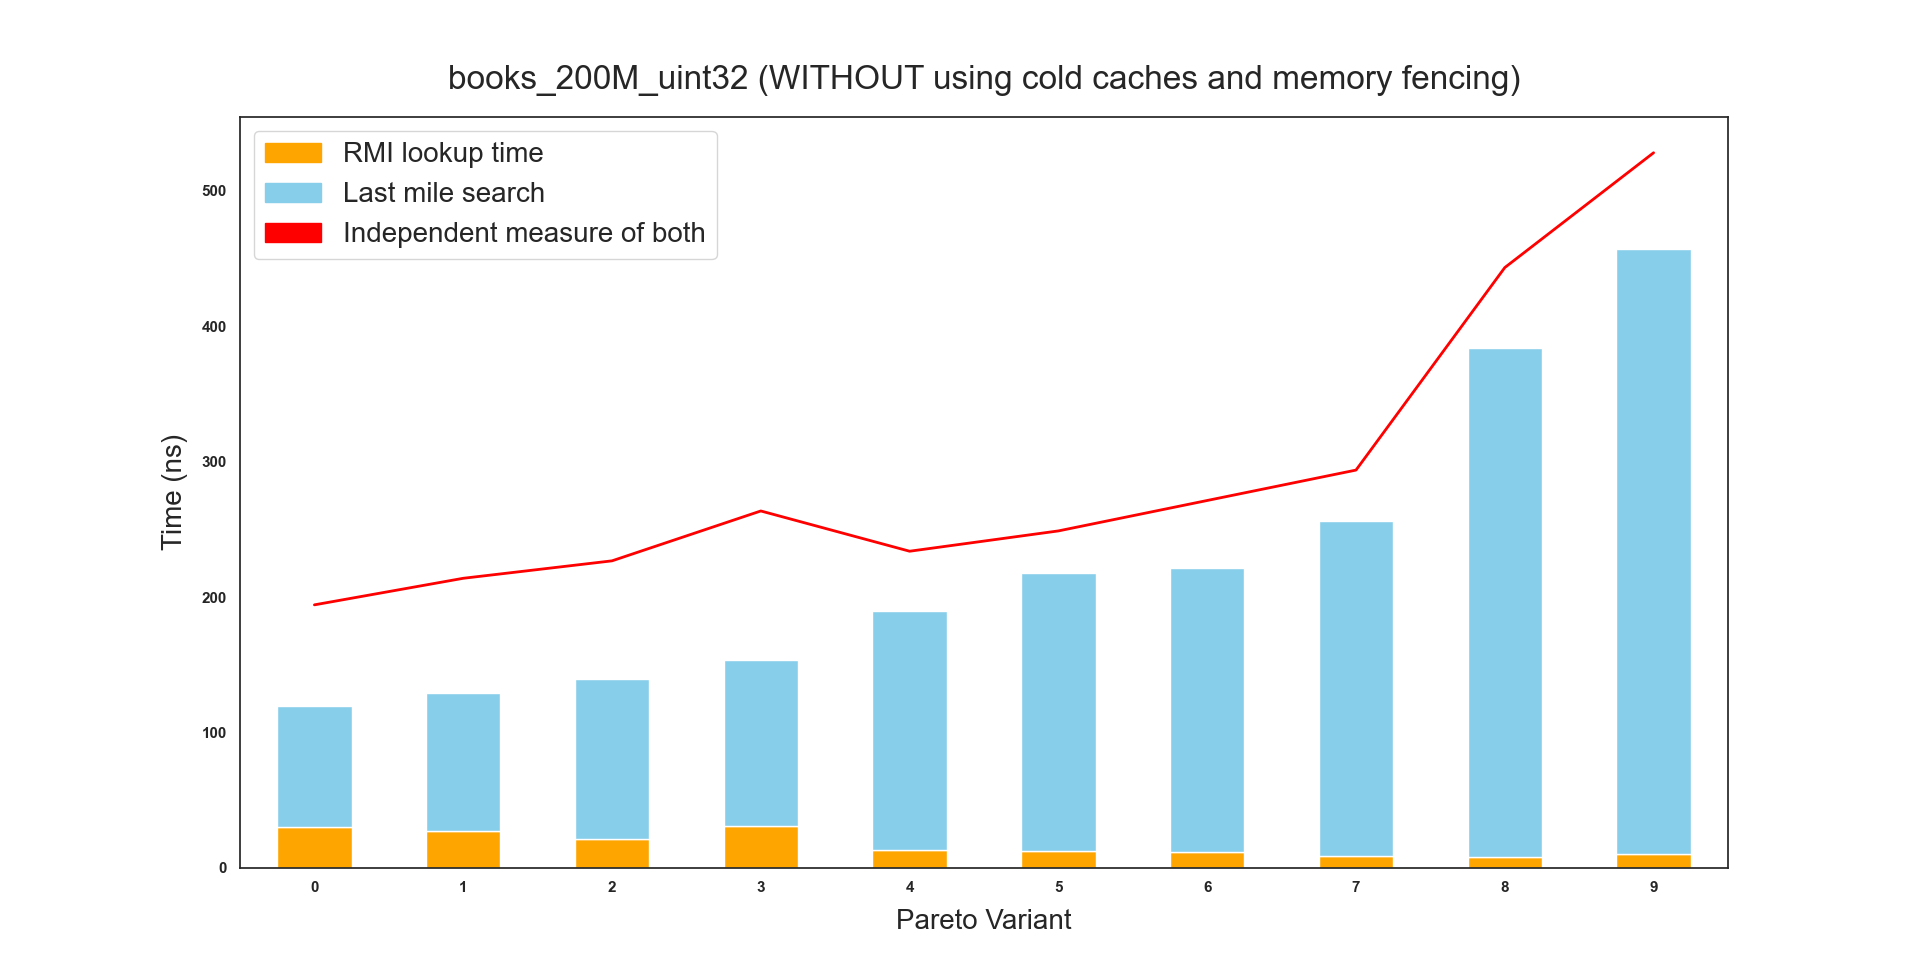
\includegraphics[width=1\textwidth]{measurements/books_200M_uint32-no-cc-mf}
  \caption[Lookup and last mile search time measures \emph{without using} cold caches and memory fencing]{
    Running the SOSD benchmark on the \emph{books\_200M\_uint32} dataset \emph{without using} cold caches or memory fencing, differentiating between pure lookup time and last mile search time.
  }
  \label{fig:books_200M_uint32-no-cc-mf}
\end{figure}

There are reasons for the way these measurements turned out which were already pointed out in section 4.4 of \cite{sosd-vldb}. Namely these reasons are that lookups in a tight loop can greatly benefit from low level CPU optimization techniques like operator reordering or caching. The same applies for the measurements in the figure above in an even more intense way, since only measuring performance of essentially lots of tightly repeated FMA instructions which the processor will optimize into a more optimal instruction order and therefore exaggerate the measured performance. The same holds true for caching, in the sense that some of the requested data will already be loaded in some cache level and therefore access time is greatly reduced.

\subsection{Using cold caches and memory fencing}
Luckily the authors of \cite{sosd-neurips} suggest and also implemented a way to mitigate these usually very desired CPU optimizations in the SOSD benchmark. The two proposed techniques aim at starting from a fresh CPU state before every lookup calculation. The first technique called cold caching mitigates cache side effects by filling the L3 CPU cache with a constant randomly generated set of numbers before each lookup. The second technique called memory fencing aims at mitigating instruction reordering by introducing memory fences before each lookup using the appropriate CPU instruction. With these techniques in place running SOSD takes a lot longer and RMI performance drastically decreases but with the advantage that more reliable meaures can be taken. The results from running the SOSD benchmark on the same dataset as previously but now using cold caches and memory fencing are shown in figure \ref{fig:books_200M_uint32}. Very similar observations can be made for all remaining 64-bit datasets provided by the SOSD benchmark shown in the appendix in section \ref{sect:appendix:measurements}.

\captionsetup[figure]{skip=10pt} % move caption down
\begin{figure}[!ht]
  \centering
  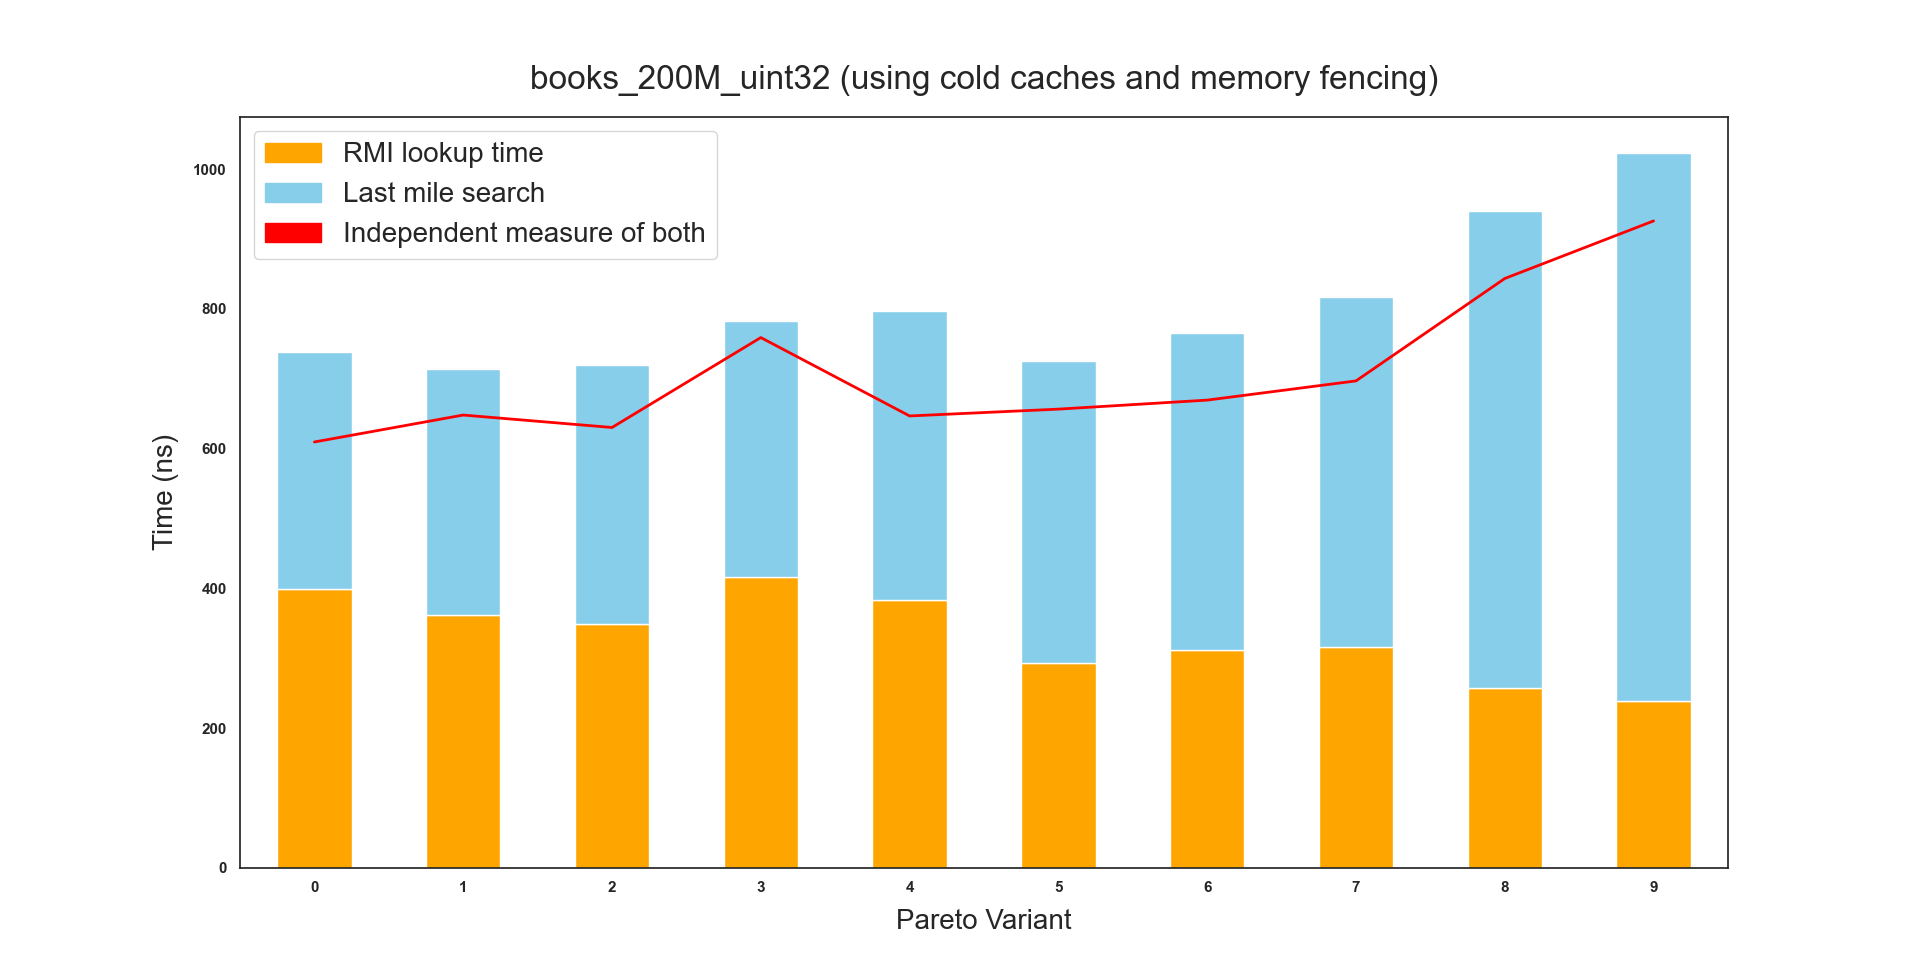
\includegraphics[width=1\textwidth]{measurements/books_200M_uint32}
  \caption[Lookup and last mile search time measures \emph{using} cold caches and memory fencing]{
    Running the SOSD benchmark on the \emph{books\_200M\_uint32} dataset \emph{using} cold caches and memory fencing, differentiating between pure lookup time and last mile search time.
  }
  \label{fig:books_200M_uint32}
\end{figure}

\subsection{Roughly approximating pure lookup time by the difference of total and last mile search time}
Finally the observation which probably leads to the best approximation of how long the pure RMI lookup operations actually take without cold caches and memory fencing, is when taking a normal measure (the red line in figure \ref{fig:books_200M_uint32-no-cc-mf}) and subtracting the last mile search time from this measure in order to guess the pure lookup operation time. This makes sense under the assumption that the last mile search code is less affected by operation reordering and caching. This is then visualized in figure \ref{fig:books_200M_uint32-no-lookup}. As for the previous experiment, similar graphs can be plotted for the remaining 64-bit datasets provided by the SOSD benchmark shown in the appendix in section \ref{sect:appendix:measurements-no-lookup}.

\captionsetup[figure]{skip=10pt} % move caption down
\begin{figure}[!ht]
  \centering
  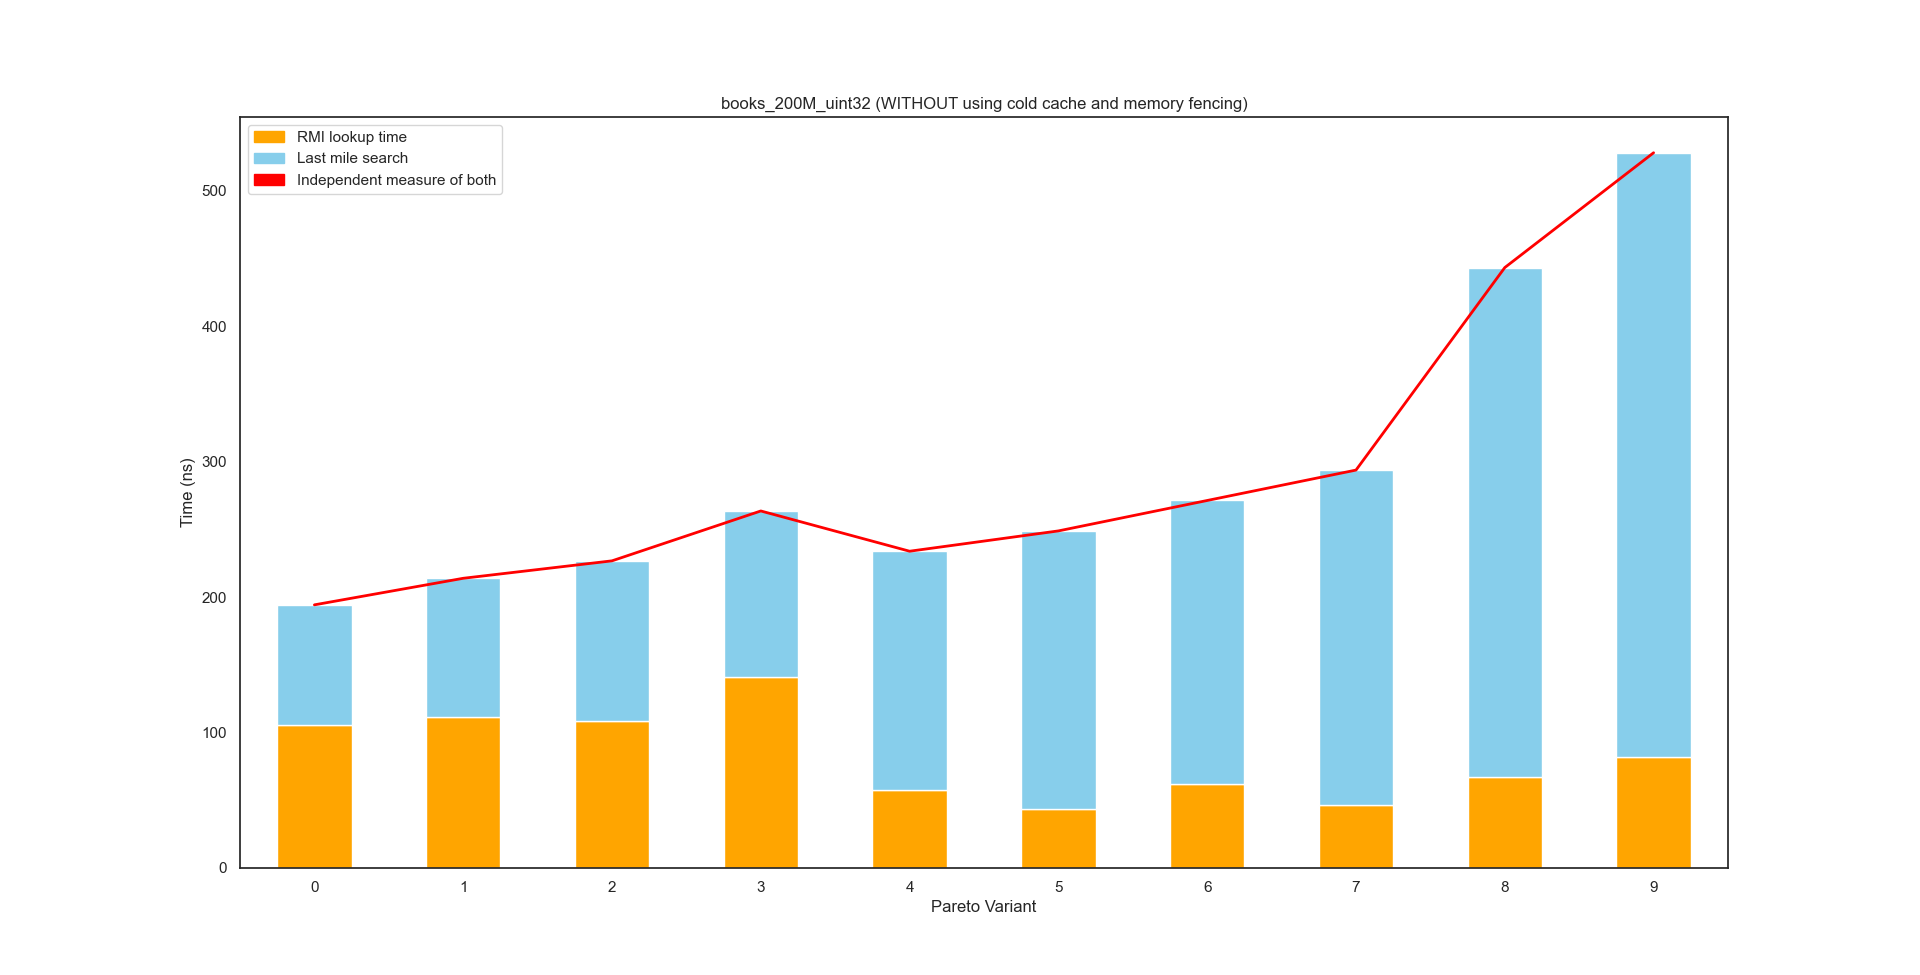
\includegraphics[width=1\textwidth]{measurements/books_200M_uint32-no-lookup}
  \caption[Last mile search time measures and lookup time approximation \emph{without using} cold caches and memory fencing]{
    Running the SOSD benchmark on the \emph{books\_200M\_uint32} dataset \emph{without using} cold caches and memory fencing, trying to approximate pure lookup time by subtracting the last mile search time from the independently measured total time.
  }
  \label{fig:books_200M_uint32-no-lookup}
\end{figure}

\subsection{Experiment observations}
When looking at the experiment figures, one can observe that the height of the blue bar (representing the last mile search time) increases with increasing pareto variant. This is expected since the SOSD benchmark trains its RMIs with decreasing index size limit relative to increasing pareto variant, meaning that with decreasing index size the last mile search bound becomes larger and therefore time spent to find a key in said larger bound increases. A next observation which is pointed out in \cite{sosd-vldb} is that the intensity at which RMI benefits from low level CPU optimizations heavily depends on many factors such as the shape of the data itself and the actual optimization capability of the processor doing the calculations. This forcibly means that any measure becomes very heavily application dependant and therefore the best advice is still to test different (learned) indexing algorithms individually in concrete applications. Still, a regular CPU can highly improve RMI performance in practice, while switches do not currently support any sort of CPU optimization techniques at this level. Concretely this means that it makes sense to compare measures from figure \ref{fig:books_200M_uint32} without any CPU optimizations at play, when directly trying to compare a server's RMI lookup performance against a switch's RMI lookup performance. Due to reasons already pointed out multiple times, this comparision is unfortunately currently not possible in practice. On the other hand, when opting for a comparision under ideal conditions, we can refer to figure \ref{fig:books_200M_uint32-no-lookup}, especially if we want to know how fast our university machine can handle last mile searches only.

\section{Evaluation}
After having described our measurement method in the first section and showing visualized results in the previous section, this section focuses on giving potential take-aways from what we measured and showing that outsourcing a learned index structure to the network can lead to a speedup. The major drawback that this work makes apparant is that there are lots of requirements currently missing in real world hardware. Namely these consist of what has been described in section \ref{sect:rmionbmv2:evaluation}.\\

Our university machine's CPU takes around 80 - 400ns for a full RMI lookup, including pure lookup operations as well as last mile search, without cold caches and memory fences (Refering to figure \ref{fig:sosd_lookups}). This means that our machine can handle between 2.5 - 12.5 million full RMI lookups per second. When now looking at the graphs in figure \ref{fig:books_200M_uint32-no-lookup} and section \ref{sect:appendix:measurements-no-lookup} we find that the pure RMI lookup calculations take pretty constantly around 50 - 100ns depending on the RMI layer configuration. Further, our university machine which would only have to deal with last mile searches and could outsource the pure lookup calculations to the switch could handle between 3 - 20 million last mile searches per second and takes around 50 - 300ns for a single last mile search.\\

All in all we find that by outsourcing the RMI calculations to the switch we can constantly gain around 50 - 100ns per lookup depending on the RMI configuration but independently of the RMI's index size and with that it's last mile search bound size, which means that without performing the RMI lookup calculations a server can constantly handle more lookups per second (since the server only has to perform the last mile searches). Further, if only a single Intel® Tofino™ 3 switch can provide pure lookup operations at a rate of around 10 billion packets per second \cite{tofino3-brief}, then this switch would easily outperform multiple magnitudes of servers working on last mile searches. This means that in a closed system the amount of speed gained, when outsourcing RMI to the network, is determined by the amount of last mile search workers. Each of them can treat more last mile searches per second and adds to the overall speedup. Additionally the constantly less time not spent on the server for calculating pure lookups would be mostly free, especially when having an application in mind where a lookup has to be sent over the network anyways. Finally, when reaching a point where a single switch cannot outperform all of the available last mile search workers anymore, horizontal scaling in terms of network switches is perfectly compatible with our RMI implementation in P4.\\

% !TEX root = ../main.tex

\chapter{Conclusion}
\label{ch:conclusion}
In this work we started by evaluating different learned index structures by their potential programmability in P4. We compared performances of different (learned) index structures using the SOSD benchmark \cite{sosd-neurips} and looked at what is possible as well as what the limits of network programmability are. We came to the conclusion that the RMI learned index structure initially proposed in \cite{rmi} is a good fit for further pursuing our idea of implementing a learned index structure in P4 in order to run lookup calculations on the fly over the network.\\

In a next step we implemented a proof of concept by hand in P4 testing it's operability on virtually simulated network hardware and found that an RMI implementation with perfect accuracy in P4 is indeed possible. At the same time though, we learned what limitations apply on real world switch hardware that do not exist in simulated hardware which proved to be crucial for our implementation. This leads to probably the most pertinent conclusion of this work, namely that in order for learned indices to become viable solutions in real world applications in the future, switches need to be able to support floating point arithmetic ideally on their ALUs or even FPUs or in some other computationally cheap form. In the same sense another limitation which we are facing, especially strengthened due to the fact that we naïvly implemented floating point arithmetic in software, is that real world switches are limited by the amount of ALU stages, meaning that chained operation complexity for a single packet is pretty quickly exploited. After having implemented a proof of concept that worked for a specific dataset and a specific RMI configuration, we further opted for a more generalizable solution, by adapting the RMI reference implementation \cite{cdfshop} in a way that P4 source code files can be generated for any input dataset and mostly any RMI configuration.\\

Finally in a last step, we tried to circumvent the fact that our implementation is theoretical and tried to estimate, how much an RMI implementation over the network could save in a closed system. We come to the conclusion that when assuming ideal conditions, where an RMI implementation in P4 exists under which a switch can operate at state-of-the-art packet processing rates in an application where a lookup has to be sent over the network anyways, our idea could potentially leverage each last mile search worker by a constant magnitude of around 50-100ns per lookup depending on the RMI layer configuration.

\pagebreak

\section{Future Work}
The continuation of this work would initially consist of finding solutions for the different limitations and assumptions that were taken in the scope of this work in order to arrive at a real world learned index structure implementation over the network. One solution for floating point arithmetic could come for instance, from an immensely interesting paper \cite{netfc} about enabling accurate floating point arithmetic on P4 capable switches in a smarter way than we did for this work. Unfortunately, the results are currently limited to 16-bit floating point arithmetic and everything beyond is left as future work. Further there is another paper \cite{maltry2021critical} which proposes an alternative implementation for finding RMI configurations that yield similar lookup times and often better build times. The result of this alternative implementation could be used as input to the P4 code generation part of our adaptation of the reference implementation. This does not immediately lead to a solution of one of the problems shown in this work, but could further leverage the performance of RMI. Finally when looking at all limitations and assumptions that we discovered during this work, most of them could either be solved or at least greatly weakened when having hardware supported floating point arithmetic. In that sense a very systems related but extremly interesting start for our future work could be to try to extend the capabilities of network switches or potentially NICs to support floating point arithmetic. The topic is currently already quite highly frequented and there are already papers \cite{inline-fpa} which pursue this exact idea of applying hardware enhancements in order to allow efficient floating point arithmetic.\\

Generally evaluating other or in the future also new learned index structures regarding their network programmability will continuously be a good starting point for our future work. In that sense pursuing the idea of having a learned index structure which does not rely on floating point arithmetic could be worth exploring.


%----------------------------------------------------------------------------------------
%	BIBLIOGRAPHY
%----------------------------------------------------------------------------------------
\printbibliography[heading=bibintoc]

%----------------------------------------------------------------------------------------
%   APPENDIX
%----------------------------------------------------------------------------------------
% !TEX root = ../main.tex

\chapter{Appendix} % Main appendix title
\label{ch:appendix}

\section{Generated C++ code for books\_200M with 32-bit keys}
\label{sect:appendix:books_200M_uint32_0}

\subsection{Header file (L0 parameters)}

\begin{C++}
namespace books_200M_uint32_0 {
  const double L0_PARAMETER0 = 0.0;
  const double L0_PARAMETER1 = 0.0;
  const double L0_PARAMETER2 = 0.003906249768078851;
  const double L0_PARAMETER3 = 0.0;
  char* L1_PARAMETERS;
}\end{C++}

\subsection{Code file (Lookup code)}

\begin{C++}
#include "books_200M_uint32_0_data.h"
#include <math.h>
#include <cmath>
#include <fstream>
#include <filesystem>
#include <iostream>
namespace books_200M_uint32_0 {
bool load(char const* dataPath) {
  {
    std::ifstream infile(std::filesystem::path(dataPath) / "books_200M_uint32_0_L1_PARAMETERS", std::ios::in | std::ios::binary);
    if (!infile.good()) return false;
    L1_PARAMETERS = (char*) malloc(402653184);
    if (L1_PARAMETERS == NULL) return false;
    infile.read((char*)L1_PARAMETERS, 402653184);
    if (!infile.good()) return false;
  }
  return true;
}
void cleanup() {
  free(L1_PARAMETERS);
}

inline double linear(double alpha, double beta, double inp) {
  return std::fma(beta, inp, alpha);
}

inline double cubic(double a, double b, double c, double d, double x) {
  auto v1 = std::fma(a, x, b);
  auto v2 = std::fma(v1, x, c);
  auto v3 = std::fma(v2, x, d);
  return v3;
}

inline size_t FCLAMP(double inp, double bound) {
  if (inp < 0.0) return 0;
  return (inp > bound ? bound : (size_t)inp);
}

uint64_t lookup(uint64_t key, size_t* err) {
  double fpred;
  size_t modelIndex;
  fpred = cubic(L0_PARAMETER0, L0_PARAMETER1, L0_PARAMETER2, L0_PARAMETER3, (double)key);
  modelIndex = (uint64_t) fpred;
  fpred = linear(*((double*) (L1_PARAMETERS + (modelIndex * 24) + 0)), *((double*) (L1_PARAMETERS + (modelIndex * 24) + 8)), (double)key);
  *err = *((uint64_t*) (L1_PARAMETERS + (modelIndex * 24) + 16));

  return FCLAMP(fpred, 200000000.0 - 1.0);
} }\end{C++}

\section{FMA operation in P4}

\subsection{Addition}
\label{sect:appendix:floating_addition}

\begin{P4}
action floating_add(in double_t first, in double_t second, out overflow128_t result) {
  bool first_bigger = first.exponent == second.exponent ? first.mantissa > second.mantissa : first.exponent > second.exponent;
  uint64_t first_mantissa = ((uint64_t) first.mantissa) | HIDDEN_BIT;
  uint64_t second_mantissa = ((uint64_t) second.mantissa) | HIDDEN_BIT;

  if ((first.exponent == 0 && first.mantissa == 0) || (second.exponent == 0 && second.mantissa == 0)) {
    if (first.exponent == 0 && first.mantissa == 0) {
      result = { second.sign, second.exponent, (bit<128>) second_mantissa }; // first zero, return second
    } else {
      result = { first.sign, first.exponent, (bit<128>) first_mantissa }; // second zero, return first
    }
    return;
  }

  exponent_t exponent_difference = first_bigger ? (first.exponent - second.exponent) : (second.exponent - first.exponent);
  uint64_t bigger_mantissa = first_bigger ? first_mantissa : second_mantissa;
  uint64_t smaller_mantissa = first_bigger ? second_mantissa : first_mantissa;
  smaller_mantissa = smaller_mantissa >> ((bit<8>) exponent_difference);

  result.sign = first_bigger ? first.sign : second.sign;
  result.exponent = first_bigger ? first.exponent : second.exponent;
  if (first.sign != second.sign) { // inputs have different sign, this is a subtraction
    result.mantissa = (bit<128>) (bigger_mantissa - smaller_mantissa);
  } else { // both numbers have the same sign, regular addition
    result.mantissa = (bit<128>) (bigger_mantissa + smaller_mantissa);
  }
}

control FloatingAdder(in double_t first, in double_t second, out double_t result) {
  FloatingNormalizer() normalizer;

  overflow128_t temp;
  apply {
    floating_add(first, second, temp);
    normalizer.apply(temp);
    result = { temp.sign, temp.exponent, (mantissa_t) temp.mantissa };
  }
}\end{P4}

\subsection{Multiplication}
\label{sect:appendix:floating_multiplication}

\begin{P4}
action floating_multiply(in double_t first, in double_t second, out overflow128_t result) {
  if ((first.exponent == 0 && first.mantissa == 0) || (second.exponent == 0 && second.mantissa == 0)) {
    result = { first.sign ^ second.sign, 0, 0 }; return;
  }

  result.sign = first.sign ^ second.sign; // ^ = xor
  result.exponent = (first.exponent - EXPONENT_BIAS) + (second.exponent - EXPONENT_BIAS) + EXPONENT_BIAS;

  bit<128> first_mantissa = ((bit<128>) first.mantissa) | (bit<128>) HIDDEN_BIT;
  bit<128> second_mantissa = ((bit<128>) second.mantissa) | (bit<128>) HIDDEN_BIT;

  result.mantissa = (first_mantissa * second_mantissa) >> 52;
}

control FloatingMultiplier(in double_t first, in double_t second, out double_t result) {
  FloatingNormalizer() normalizer;

  overflow128_t temp;
  apply {
    floating_multiply(first, second, temp);
    normalizer.apply(temp);
    result = { temp.sign, temp.exponent, (mantissa_t) temp.mantissa };
  }
}\end{P4}

\subsection{Normalization}
\label{sect:appendix:floating_normalization}

\begin{P4}
control FloatingNormalizer(inout overflow128_t overflow) {
  action floating_shift_left(inout overflow128_t result, bit<8> amount) {
    result.mantissa = result.mantissa << amount;
    result.exponent = result.exponent - (exponent_t) amount;
  }

  action floating_shift_right(inout overflow128_t result, bit<8> amount) {
    result.mantissa = result.mantissa >> amount;
    result.exponent = result.exponent + (exponent_t) amount;
  }

  table floating_normalize {
    key = {
      overflow.mantissa: ternary;
    }
    actions = {
      floating_shift_left(overflow);
      floating_shift_right(overflow);
      NoAction;
    }
    const default_action = NoAction();
    const entries =  { // value to match against &&& bit mask
      0b1000...0 &&& 0b100...0: floating_shift_right(overflow, 75);
      0b0100...0 &&& 0b110...0: floating_shift_right(overflow, 74);
      0b0010...0 &&& 0b111...0: floating_shift_right(overflow, 73);
      // ...
      // the mask where the first significant bit is at pos 53 needs no action
      // ...
      0b0...0100 &&& 0b1...100: floating_shift_left(overflow, 50);
      0b0...0010 &&& 0b1...110: floating_shift_left(overflow, 51);
      0b0...0001 &&& 0b1...111: floating_shift_left(overflow, 52);
    }
  }

  apply {
      floating_normalize.apply();
  }
}\end{P4}

\subsection{FMA}
\label{sect:appendix:fma}

\begin{P4}
control FloatingFusedMultiplyAdd(in double_t x, in double_t y, in double_t z, out double_t result) {
  FloatingAdder() adder_instance;
  FloatingMultiplier() multiplier_instance;

  apply {
    multiplier_instance.apply(x, y, result);
    adder_instance.apply(result, z, result);
  }
}\end{P4}

\section{Loading model parameters}

\subsection{Data plane RMI table declaration in P4}
\label{sect:appendix:rmi_table}

\begin{P4}
control ModelLookup(in uint64_t model_index, out double_t first_l1, out double_t second_l1, out uint64_t err) {

  action assign_variables(sign_t first_sign, exponent_t first_exponent, mantissa_t first_mantissa,
                          sign_t second_sign, exponent_t second_exponent, mantissa_t second_mantissa,
                          uint64_t err_val) {
      first_l1 = { first_sign, first_exponent, first_mantissa };
      second_l1 = { second_sign, second_exponent, second_mantissa };
      err = err_val;
  }

  table model_lookup {
      key = {
          model_index: exact;
      }
      actions = {
          assign_variables;
          NoAction;
      }
      const default_action = assign_variables(0, 0, 0, 0, 0, 0, 0);
      const size = 550000; // depends on model parameter size
  }
  apply {
      assign_variables(0, 0, 0, 0, 0, 0, 0);
      model_lookup.apply();
  }
}\end{P4}

\subsection{Control plane batch sending of model parameters in Python}
\label{sect:appendix:sending_params}

\begin{python}
BATCH_SIZE = 2048

SIGN_MASK = 0x8000000000000000
EXPONENT_MASK = 0x7FF0000000000000
MANTISSA_MASK = 0x000FFFFFFFFFFFFF

def writeL1Parameters(p4info_helper, switch):
  if not os.path.exists('path/to/layer_parameters'): print('Parameters file not found!'); return
  model_index = 0
  with open('path/to/layer_parameters', 'rb') as file:
    bytes = file.read(24 * BATCH_SIZE)
    while bytes:
      entries_batch = []
      for index in range(0, BATCH_SIZE):
        model_bytes = bytes[(24 * index):(24 * (index + 1))]
        first_l1 = int.from_bytes(model_bytes[0:8], byteorder='little')
        second_l1 = int.from_bytes(model_bytes[8:16], byteorder='little')
        third_l1 = int.from_bytes(model_bytes[16:24], byteorder='little')

        table_entry = p4info_helper.buildTableEntry(
          table_name='LearnedIngress.lookup_instance.l1_lookup.l1_model_lookup',
          match_fields={ 'model_index': model_index },
          action_name='LearnedIngress.lookup_instance.l1_lookup.assign_variables',
          action_params={
            'first_l1_sign': (first_l1 & SIGN_MASK) >> 63,
            'first_l1_exponent': (first_l1 & EXPONENT_MASK) >> 52,
            'first_l1_mantissa': first_l1 & MANTISSA_MASK,
            'second_l1_sign': (second_l1 & SIGN_MASK) >> 63,
            'second_l1_exponent': (second_l1 & EXPONENT_MASK) >> 52,
            'second_l1_mantissa': second_l1 & MANTISSA_MASK,
            'third_l1_input': third_l1
          })
        entries_batch.append(table_entry)
        model_index += 1

      switch.WriteTableEntries(entries_batch)
      bytes = file.read(24 * BATCH_SIZE)\end{python}

\section{RMI lookup fuction in P4}

\begin{P4}
control LearnedLookup(in double_t input_key, out uint64_t guess, out uint64_t guess_err) {
  ModelLookup() lookup_instance;
  LearnedCubic() cubic_instance;
  LearnedLinear() linear_instance;

  double_t fpred;
  uint64_t model_index;
  double_t first_l1; double_t second_l1;

  apply {
    // 1. using static L0 parameters as input for the first cubic model layer
    cubic_instance.apply({ 0, 0, 0 }, { 0, 0, 0 }, { 0, 1014, 4503599092596736 }, { 0, 0, 0 }, input_key, fpred);
    double_to_int(fpred, model_index);

    lookup_instance.apply(model_index, first_l1, second_l1, guess_err); // 2. retrieving L1 parameters

    // 3. using retrieved L1 parameters as input for second linear model layer
    linear_instance.apply(first_l1, second_l1, input_key, fpred);
    double_to_int(fpred, guess);

    f_clamp(fpred, 0xbebc1ff, guess);
  }
}\end{P4}

\newpage % ugly, but otherwise latex does not place section title correctly

\section{Experiment results using cold caches and memory fencing}
\label{sect:appendix:measurements}

\captionsetup[figure]{skip=10pt} % move caption down
\begin{figure}[!htb]
  \centering
  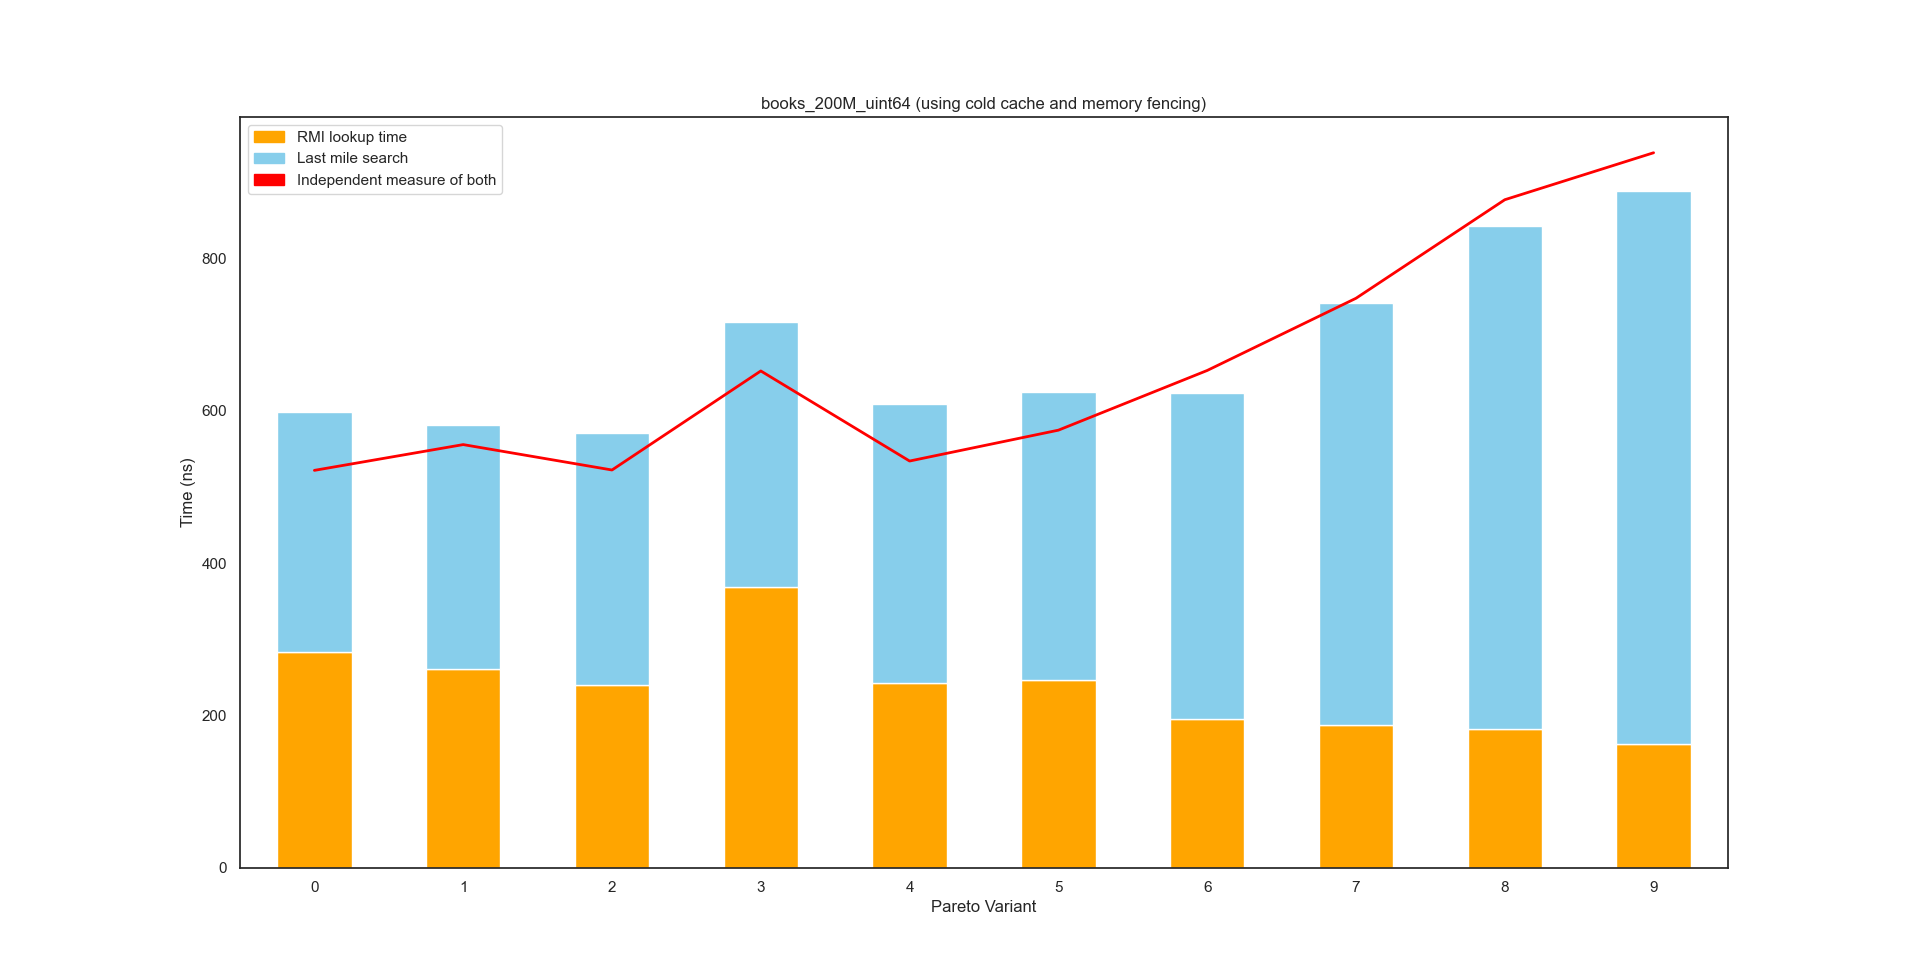
\includegraphics[width=1\textwidth]{measurements/books_200M_uint64}
  \caption*{
    Running the SOSD benchmark on the \emph{books\_200M\_uint64} dataset \emph{using} cold caches and memory fencing, differentiating between pure lookup time and last-mile search time.
  }
\end{figure}

\begin{figure}[!htb]
  \centering
  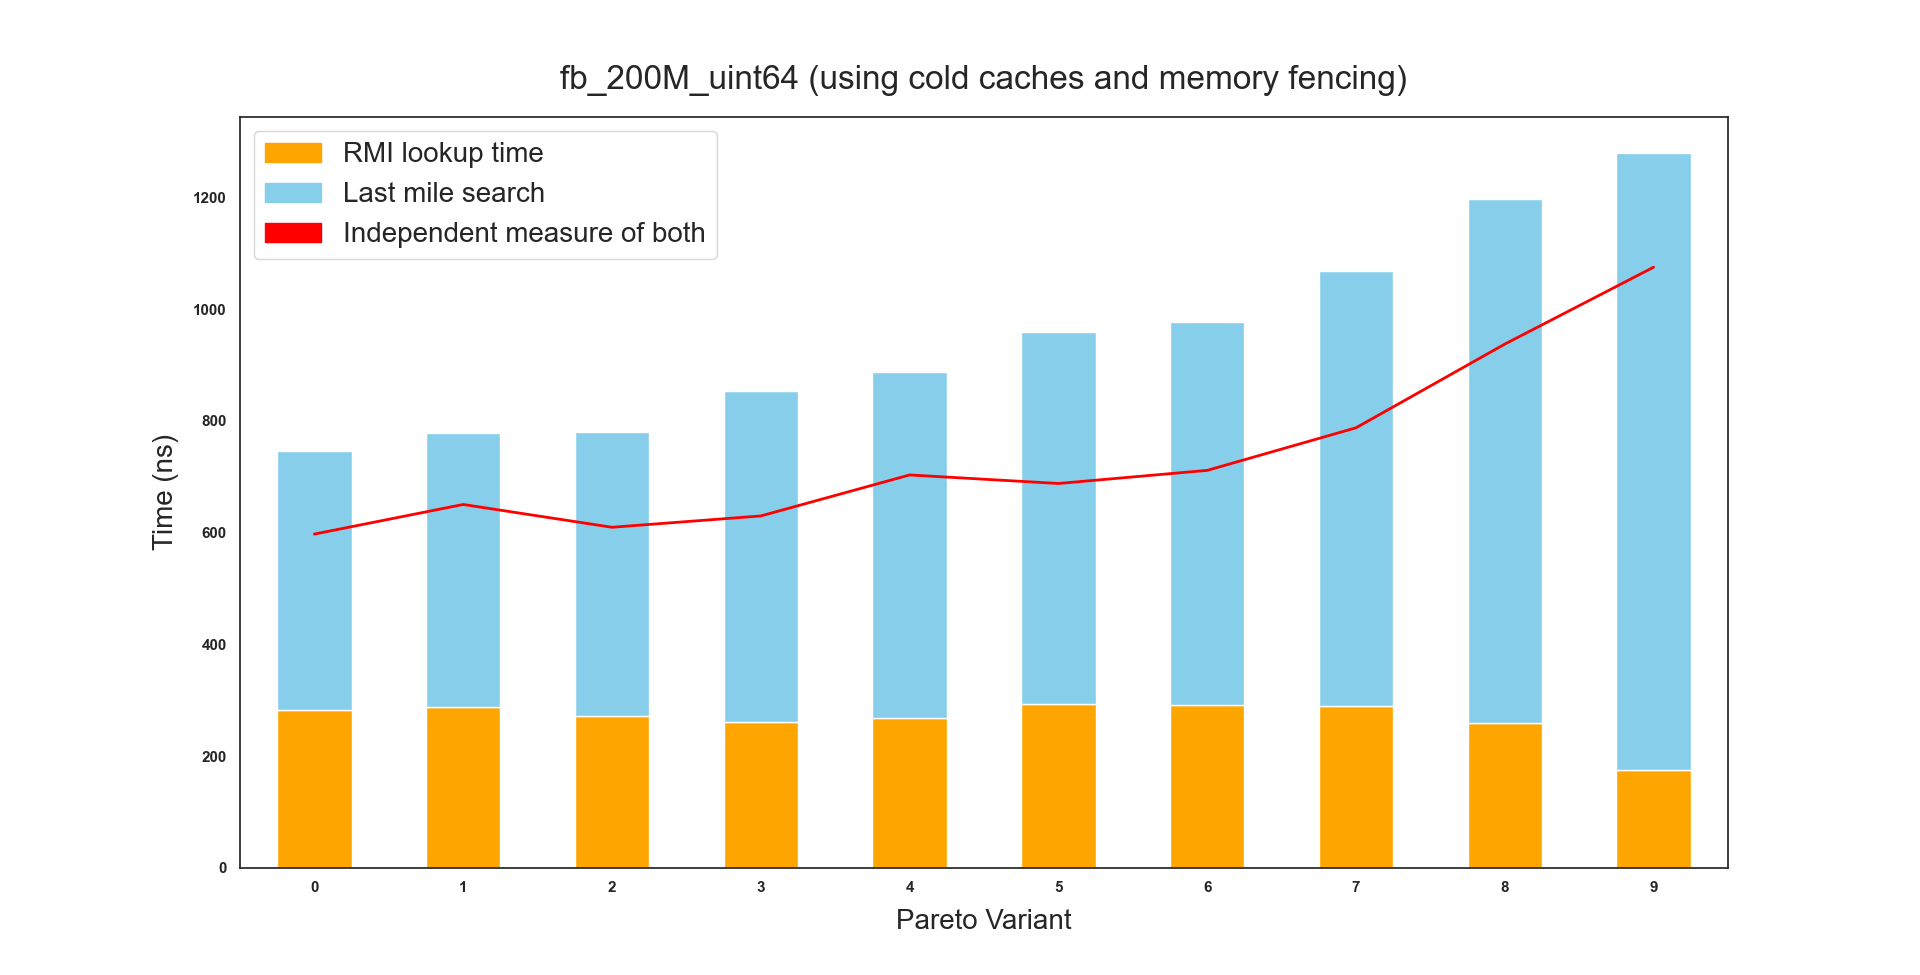
\includegraphics[width=1\textwidth]{measurements/fb_200M_uint64}
  \caption*{
    Running the SOSD benchmark on the \emph{fb\_200M\_uint64} dataset \emph{using} cold caches and memory fencing, differentiating between pure lookup time and last-mile search time.
  }
\end{figure}

\begin{figure}[!htb]
  \centering
  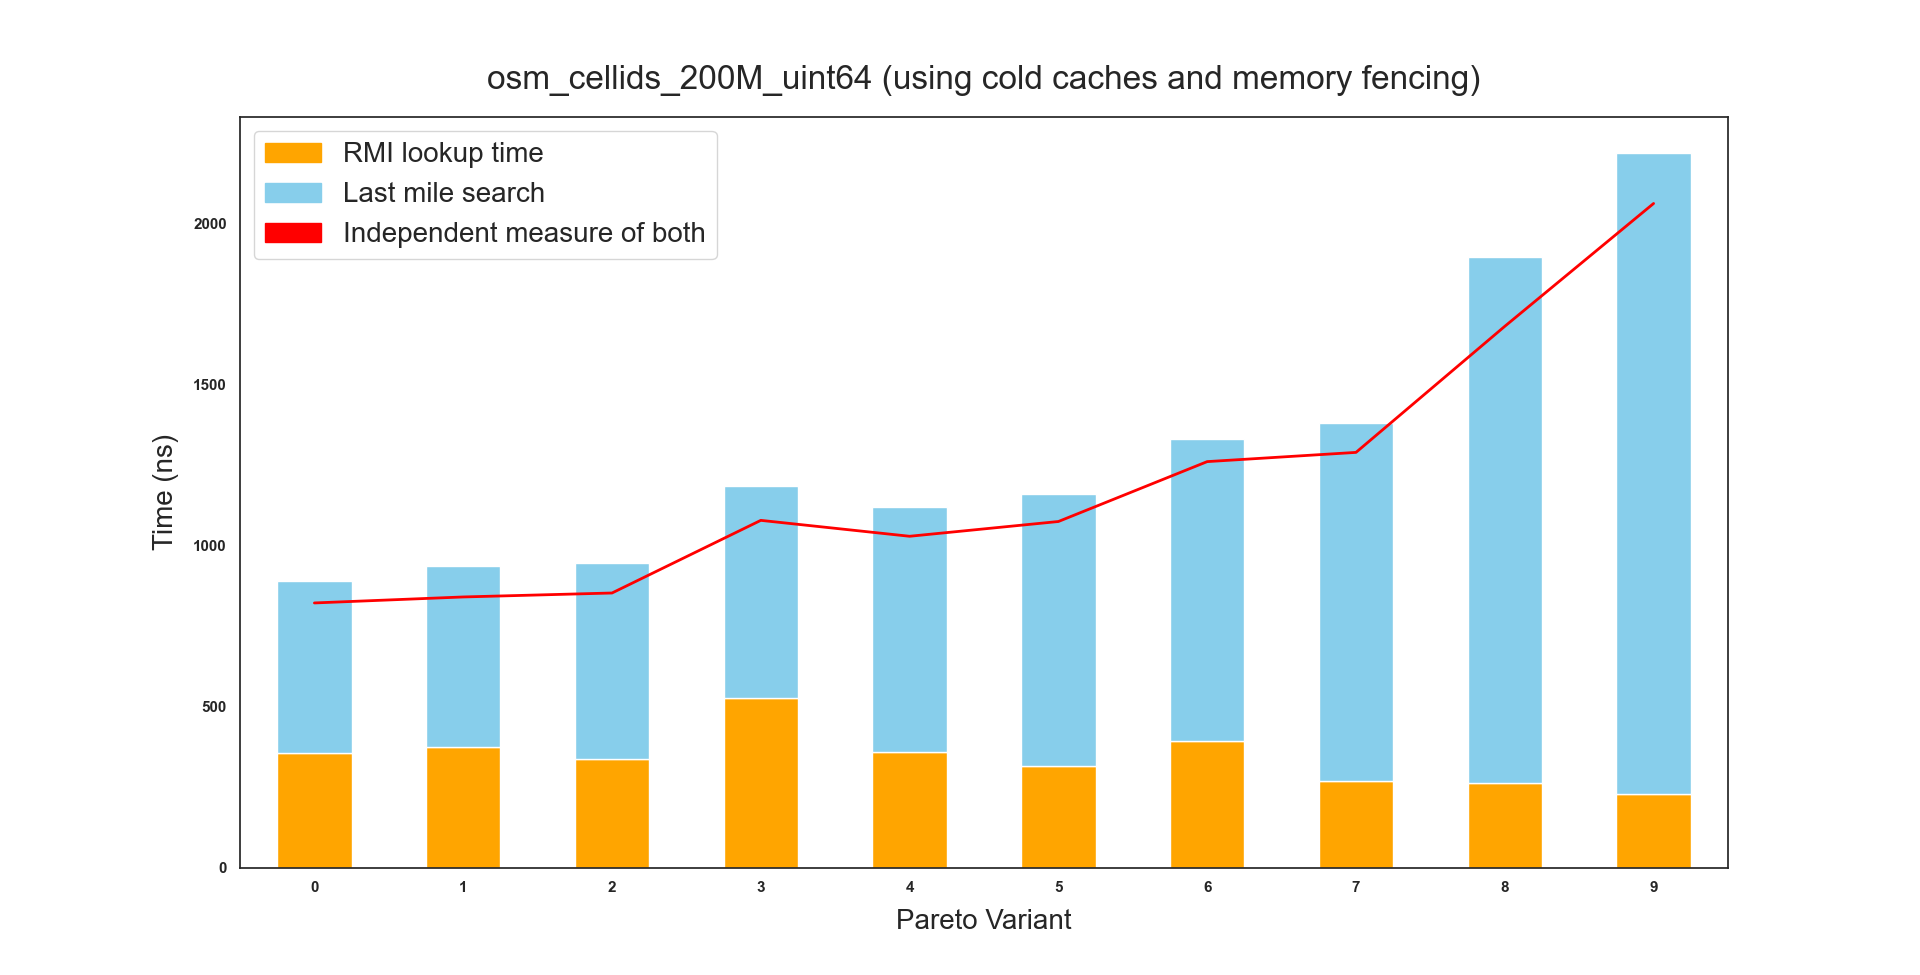
\includegraphics[width=1\textwidth]{measurements/osm_cellids_200M_uint64}
  \caption*{
    Running the SOSD benchmark on the \emph{osm\_cellids\_200M\_uint64} dataset \emph{using} cold caches and memory fencing, differentiating between pure lookup time and last-mile search time.
  }
\end{figure}

\begin{figure}[!htb]
  \centering
  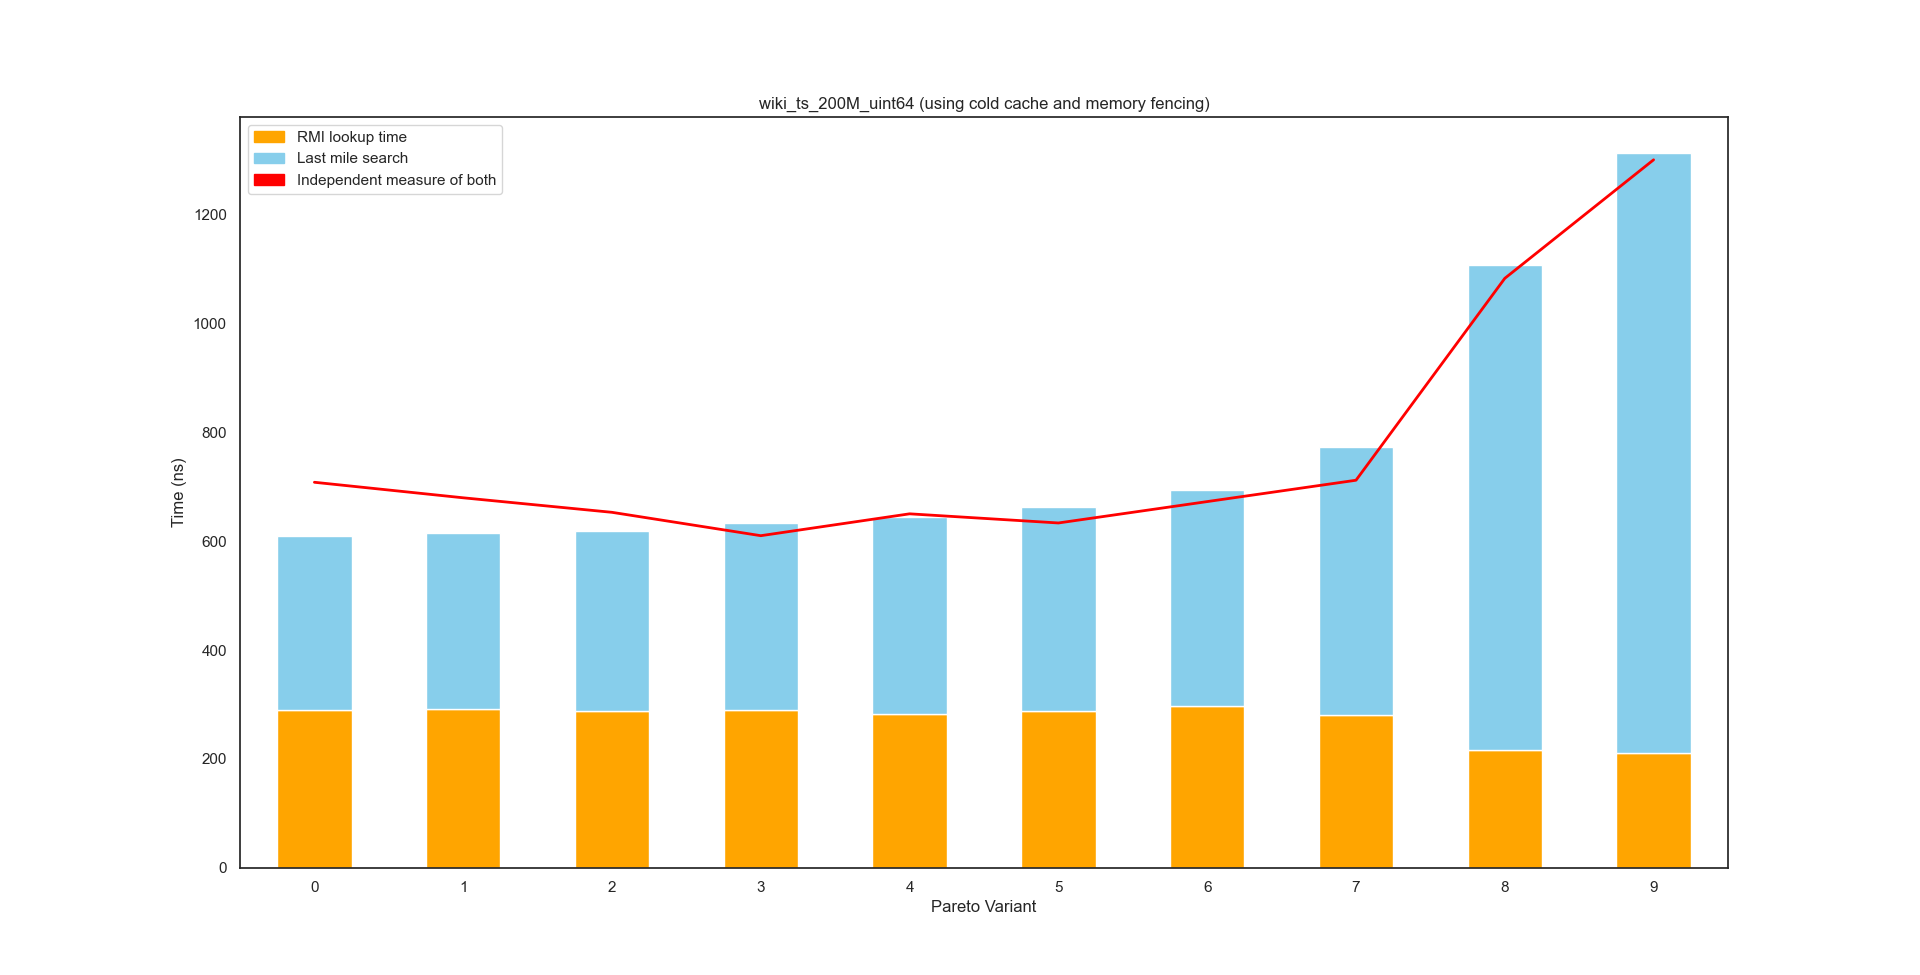
\includegraphics[width=1\textwidth]{measurements/wiki_ts_200M_uint64}
  \caption*{
    Running the SOSD benchmark on the \emph{wiki\_ts\_200M\_uint64} dataset \emph{using} cold caches and memory fencing, differentiating between pure lookup time and last-mile search time.
  }
\end{figure}

\newpage % ugly, but otherwise latex does not place section title correctly

\section{Experiment results calculating pure lookup time as the difference of the total time measured and last-mile search time}
\label{sect:appendix:measurements-no-lookup}

\captionsetup[figure]{skip=10pt} % move caption down
\begin{figure}[!htb]
  \centering
  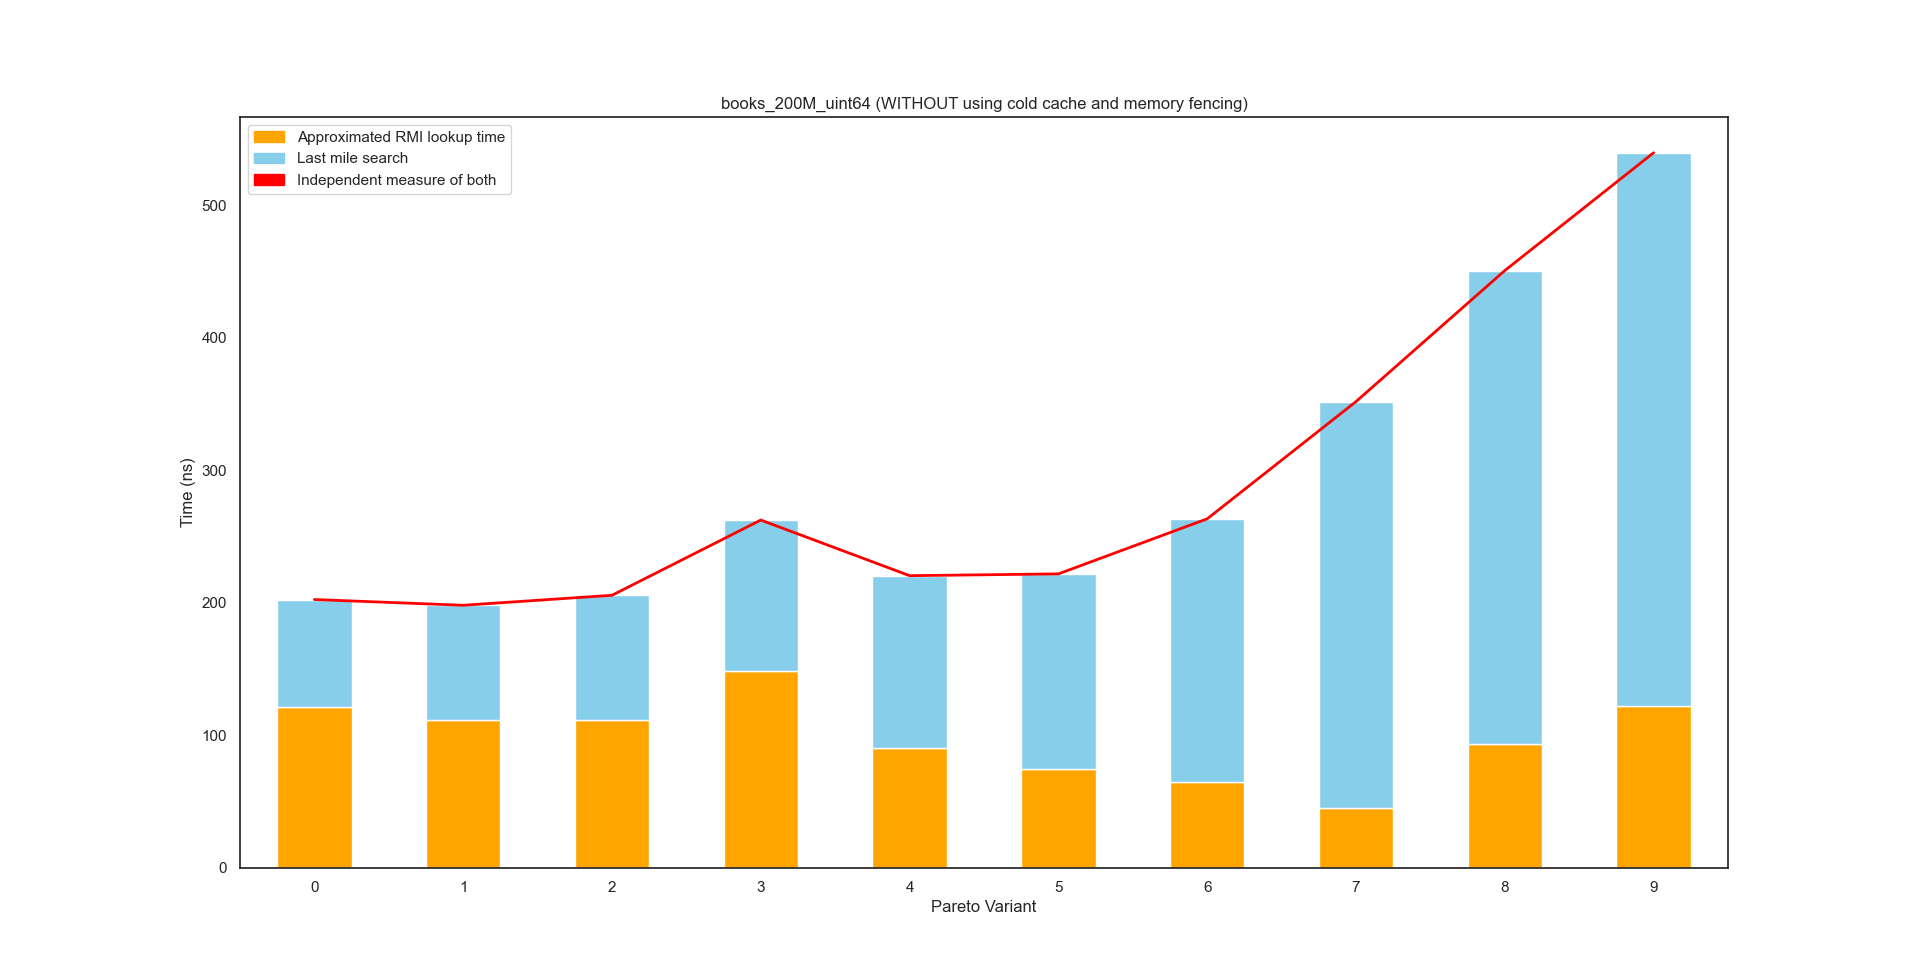
\includegraphics[width=1\textwidth]{measurements/books_200M_uint64-no-lookup}
  \caption*{
    Running the SOSD benchmark on the \emph{books\_200M\_uint64} dataset \emph{without using} cold caches and memory fencing, trying to approximate pure lookup time by subtracting last-mile search time from the totally measured time.
  }
\end{figure}

\begin{figure}[!htb]
  \centering
  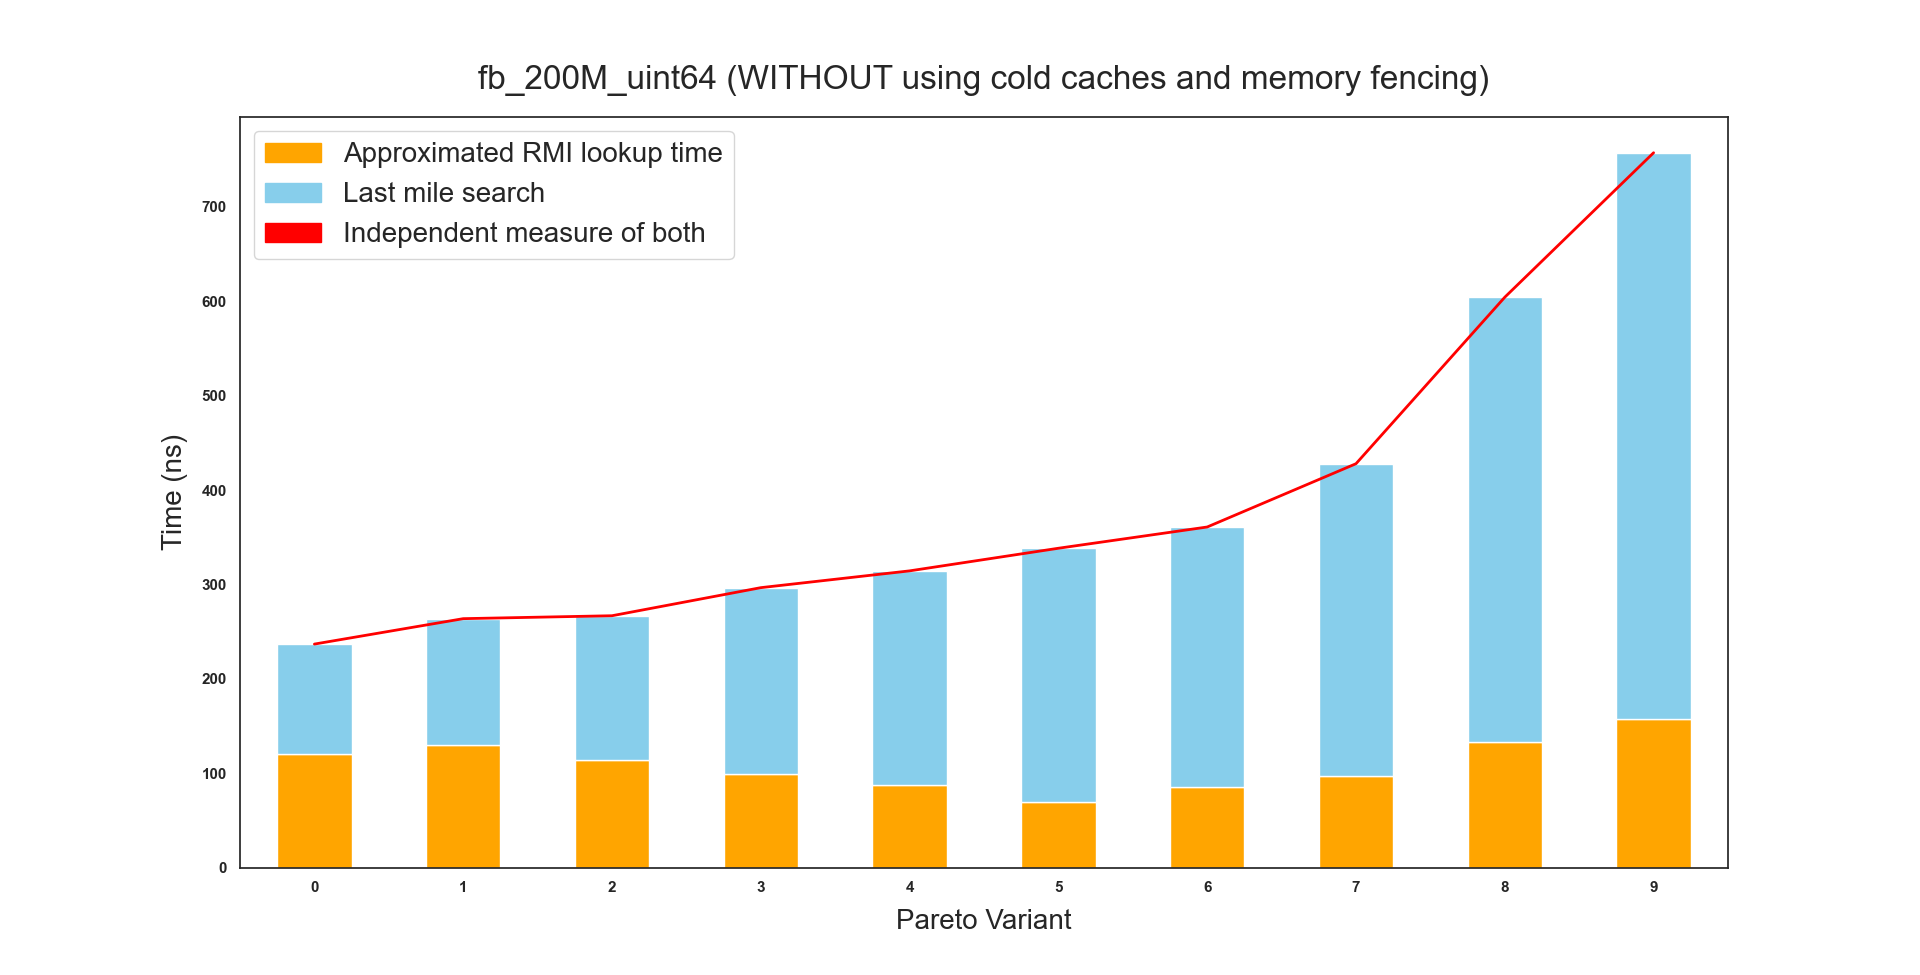
\includegraphics[width=1\textwidth]{measurements/fb_200M_uint64-no-lookup}
  \caption*{
    Running the SOSD benchmark on the \emph{fb\_200M\_uint64} dataset \emph{without using} cold caches and memory fencing, trying to approximate pure lookup time by subtracting last-mile search time from the totally measured time.
  }
\end{figure}

\begin{figure}[!htb]
  \centering
  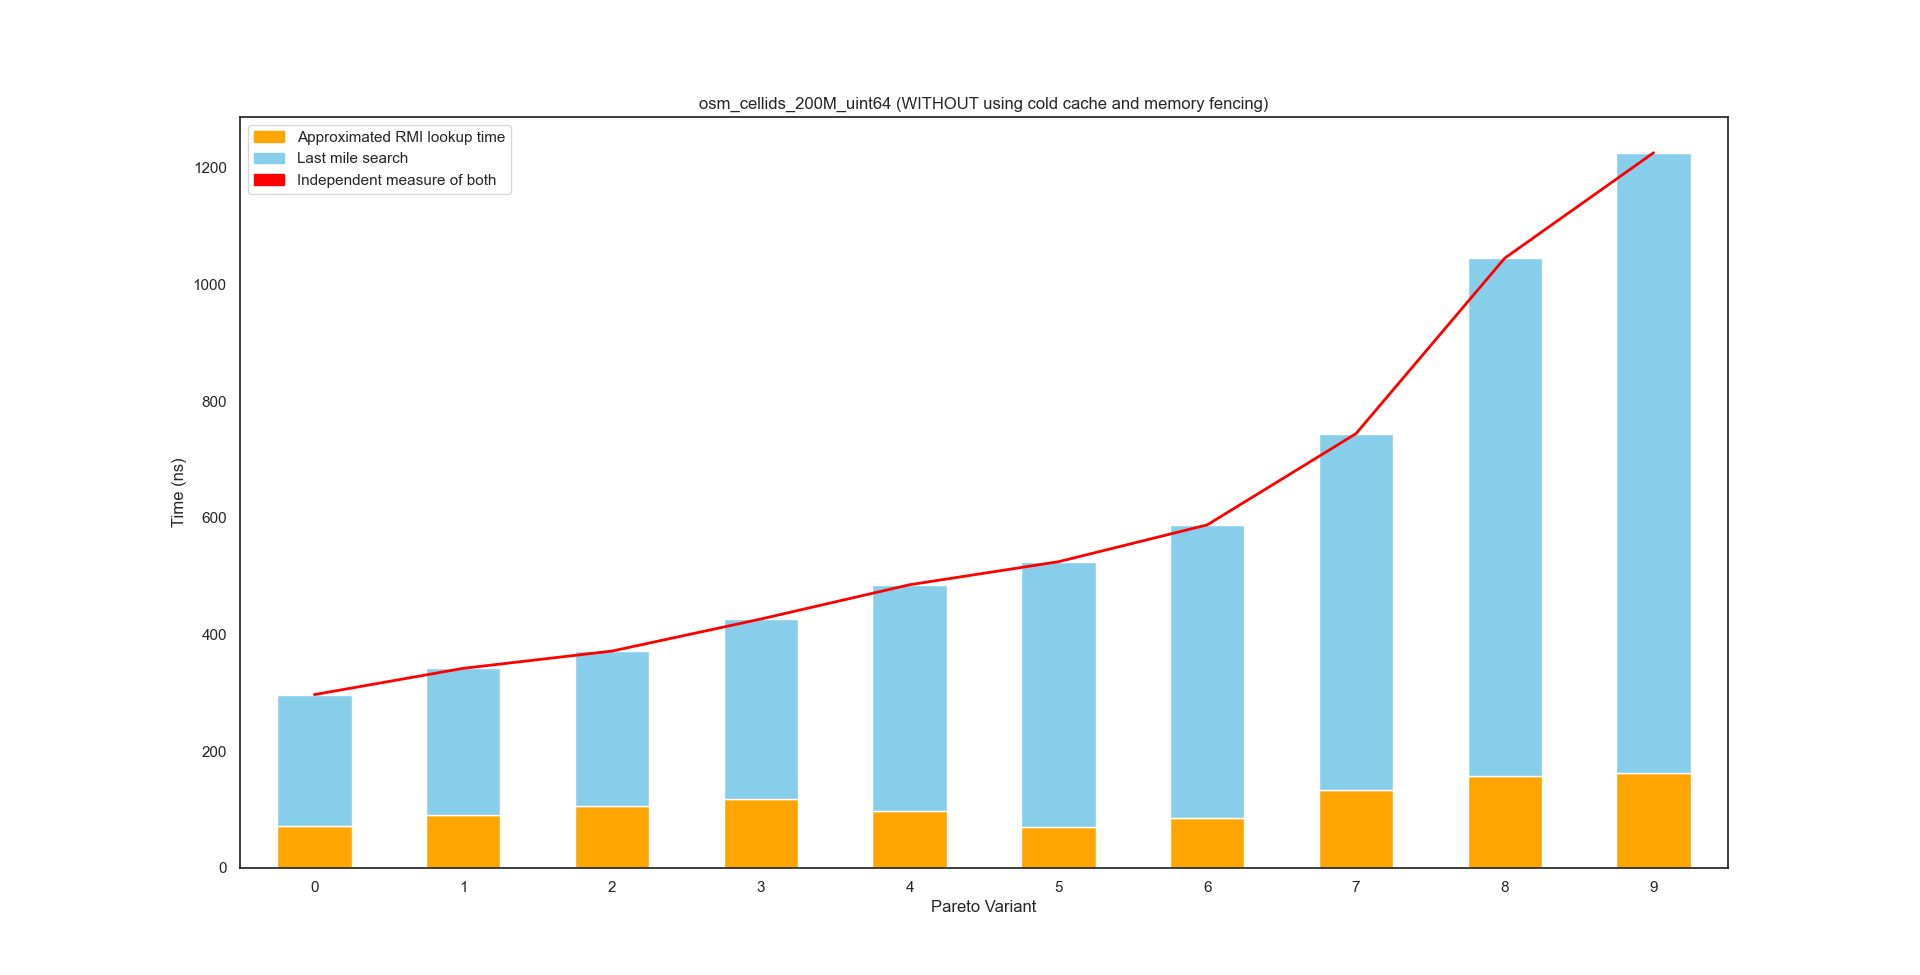
\includegraphics[width=1\textwidth]{measurements/osm_cellids_200M_uint64-no-lookup}
  \caption*{
    Running the SOSD benchmark on the \emph{osm\_cellids\_200M\_uint64} dataset \emph{without using} cold caches and memory, fencing trying to approximate pure lookup time by subtracting last-mile search time.
  }
\end{figure}

\begin{figure}[!htb]
  \centering
  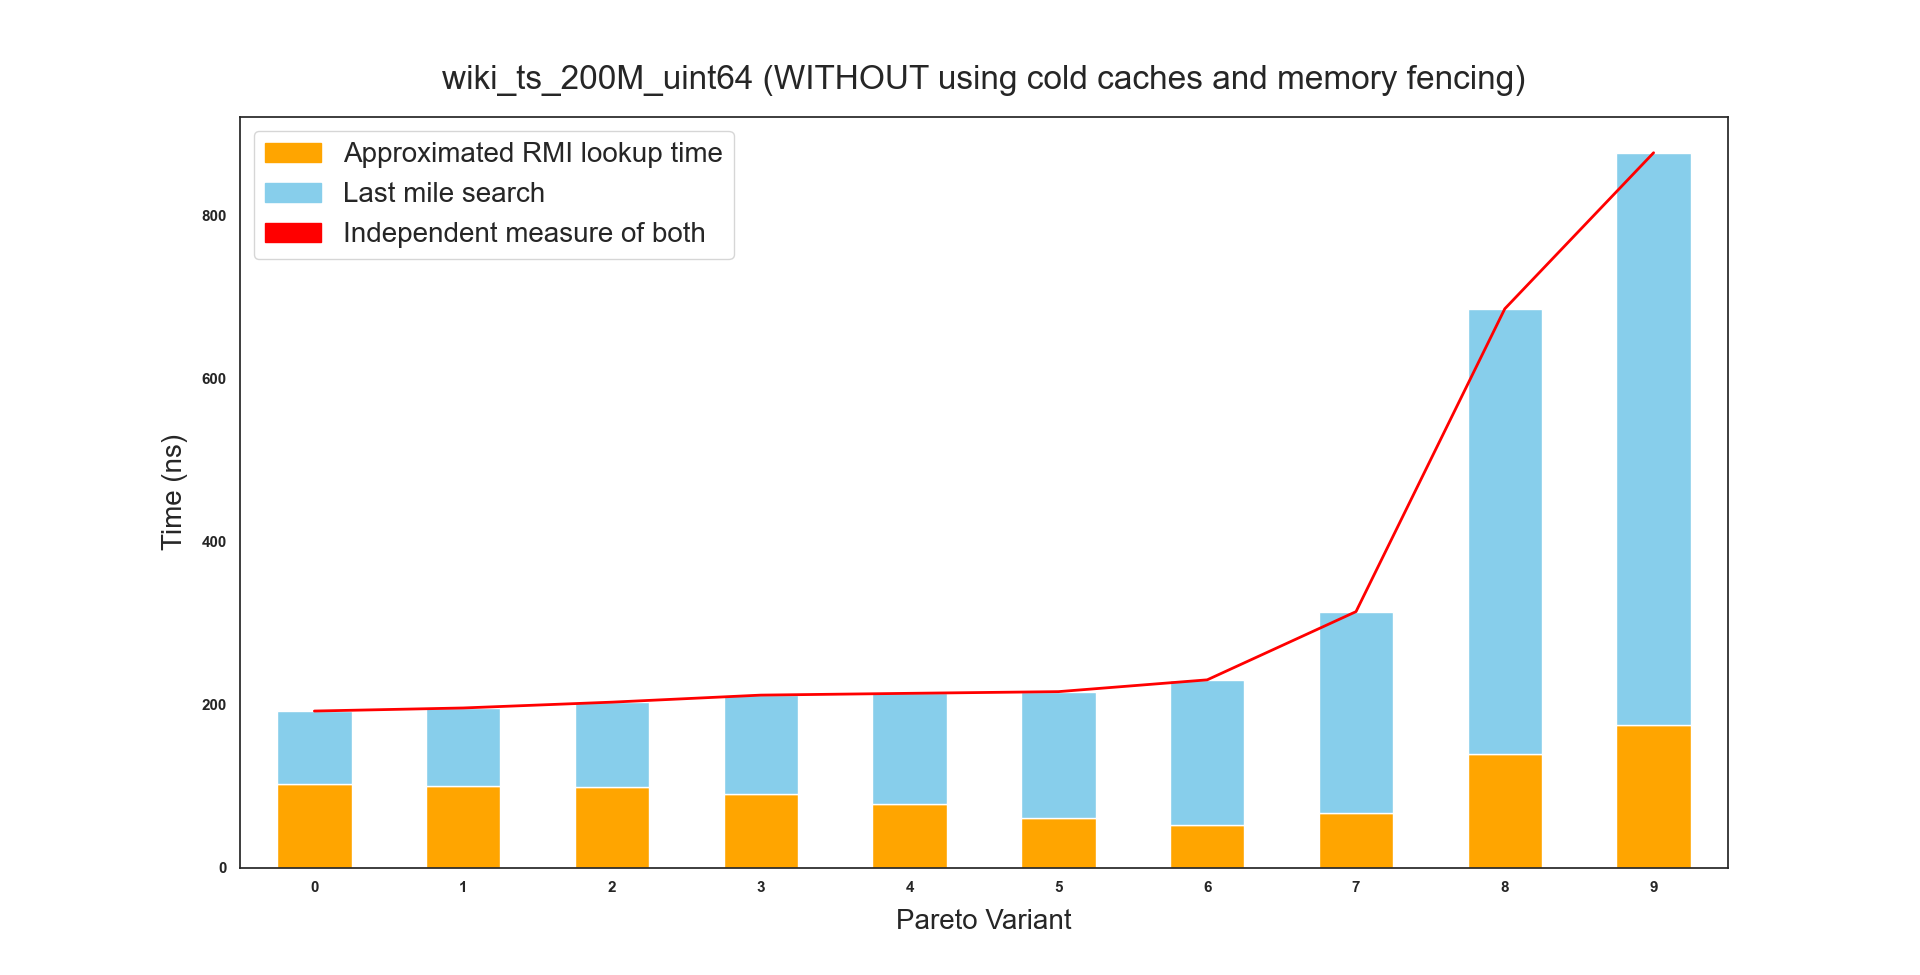
\includegraphics[width=1\textwidth]{measurements/wiki_ts_200M_uint64-no-lookup}
  \caption*{
    Running the SOSD benchmark on the \emph{wiki\_ts\_200M\_uint64} dataset \emph{without using} cold caches and memory fencing, trying to approximate pure lookup time by subtracting last-mile search time from the totally measured time.
  }
\end{figure}


%----------------------------------------------------------------------------------------
\end{document}
